\documentclass[11pt,a4paper,leqno]{report}
\usepackage{tikz}
\usepackage[USenglish]{babel}
\usepackage{amsmath}
\usepackage{amsthm}
\usepackage{amssymb}
\usepackage{float}
\usepackage{amsfonts}
\usepackage{hyperref}
%\usepackage{mathabx}
%\usepackage{makeidx}
%\usepackage{graphicx}
%\graphicspath{{pics/}}


\newcommand{\Cross}{\mathbin{\tikz [x=1.4ex,y=1.4ex,line width=.2ex] \draw (0,0) -- (1,1) (0,1) -- (1,0);}}%
\newcommand{\eps}{\varepsilon}
\newcommand{\R}{\mathbb{R}}
\newcommand{\C}{\mathbb{C}}


%%%%%%%%%%% REST %%%%%%%%%%%%%%%%%%%%%%%%%%%%%%%%%%%%

\DeclareMathOperator{\dom}{dom}
\DeclareMathOperator{\ran}{ran}
\newcommand{\re}{\mathrm{Re}}
\newcommand{\im}{\mathrm{Im}}

\newcommand{\ul}{\underline}
\newcommand{\I}{\mathrm{i}}
\newcommand{\E}{\mathrm{e}}

%\makeindex
%\setlength{\parindent}{0em} 


\newtheorem{theorem}{Theorem}[chapter]
\newtheorem{proposition}{Proposition}[chapter]
\newtheorem{lemma}[theorem]{Lemma}
\newtheorem{definition}[theorem]{Definition}
\newtheorem{corollary}[theorem]{Corollary}
\newtheorem{remark}[theorem]{Remark}

\numberwithin{equation}{chapter}




\begin{document}


\begin{titlepage}
\begin{figure}[H]
\begin{flushright}
	 \includegraphics{RZ_Logo_Uni_sw_01.jpg}
\end{flushright}
\end{figure}

\begin{center}
\Huge\bfseries Masterarbeit\\[3cm]
\small
Titel der Masterarbeit\\[0.3cm]

\huge\bfseries Constructive Rellich Compactness\\[3cm]
\small
verfasst von\\[0.3cm]
Oliver \textsc{Sko\v{c}ek} BSc.\\[2cm]
angestrebter akademischer Grad\\[0.3cm]
Master of Science (MSc.)

\end{center}
\begin{flushleft}
Wien, 2015\\[1cm]
\small
\emph{Studienkennzahl lt. Studienblatt}: A 066 821 \\[0.3cm]
\small
\emph{Studienrichtung lt. Studienblatt}: Masterstudium Mathematik UG2002\\[0.5cm]
\normalsize
\emph{Betreuer}: \bfseries Ph.D. Ilaria \textsc{Perugia}
% Bottom of the page
\end{flushleft}

 
 
\end{titlepage}

%\maketitle


%\renewcommand{\contentsname}{Contents}

\vfill
\thispagestyle{empty}
\newpage
\renewcommand{\abstractname}{Acknowledgements}
\begin{abstract}
First and foremost I would like to thank Prof. Perugia for supervising my thesis. Even though the Dirichlet problem is one of the topics she is very familiar with, constructive mathematics wasn't one of them and I am very thankful to her for taking the time and effort necessary to supervise my thesis.\\
\\
I would also like to thank Prof. Haslinger for giving me a push in the right direction, when I was still not sure how to arrive at the final result of this thesis.\\
\\
Finally I want to thank my parents, my friends and everyone  who supported me during my studies either intellectually, economically or emotionally.
\end{abstract}
\thispagestyle{empty}
\tableofcontents

\markboth{Contents}{Contents}
\vfill
\thispagestyle{empty}
\newpage
\pagenumbering{roman}
\setcounter{page}{1}
\newpage

\clearpage

\chapter*{Introduction}
\addcontentsline{toc}{chapter}{Introduction}
In my sixth semester I was particularly interested in the representation theory of von-Neumann-algebras and the theory of Schr\"odinger-operators. During that time a good friend of mine who studied physics challenged me on some of the theorems discussed in a functional analysis course I took at the time. He doubted that the theorems can be of any practical use. At first I completely denied that, but accepted the challenge to prove him wrong. So I showed him one particular theorem that in my opinion could be useful, at least for a physicist. It was Gelfand's representation theorem of abelian $C^*$-algebras and as a consequence the continuous functional-calculus. He was quite impressed by it, but doubted that the theorem had any numerical content. As a consequence I tried to come up with a constructive proof of Gelfand's representation theorem. The classical proof of this theorem relies on the existence of maximal ideals by an application of Zorn's lemma, which of course is a non-constructive theorem. At some point I came across Brouwer's Intuitionism and dismissed it immediately after I read that the law of excluded middle is rejected in intuitionistic mathematics. A short time after that I found the Wikipedia article on "Specker sequences" and was shocked to realize that the least-upper-bound-principle, Heine-Borel and Bolzano-Weierstrass fail to hold in a computational sense. This was the first \textbf{Brouwerian counterexample }I encountered and I wish to share it with the reader.\\
\\
Before I can do that, I need to define a few things and give a few explanations for the reader not familiar with computability theory. There are a lot of different notions of computability. A few of them like for example the notion of \textbf{recursive functions} and \textbf{Turing machines} can emulate any, according to any other known definition of computability, computable function. In fact there is no known computable function, that is not recursive or equivalently can be represented as a Turing machine. This does not mean that there cannot be any, we just don't know, but we shall assume it for this example. A set $B\subset\mathbb{N}$ is called \textbf{recursive} if there exists a computer program that can decide in a finite amount of time whether or not a given natural number belongs to $B$. If on the other hand there is only a computer program that given $n\in\mathbb{N}$ will either after a finite amount of time halt and say "yes, n belongs to B" if $n$ is in fact an element of $B$ or otherwise run forever, then the set $B$ is called \textbf{recursively enumerable}. Like the name suggests if a set $B$ is recursively enumerable then we can use this to write a computer program, that enumerates $B$. Obviously a set $B\subset\mathbb{N}$ is recursive if and only if $B$ and $B^c$ are recursively enumerable.\\ 
\\
The important question now is whether or not there is an example of a recursively enumerable set that is not recursive. 
Before I answer this question let me introduce the notion of a \textbf{G\"odel enumeration}. A program in a given programming language is a finite sequence of elementary instructions. Given a programming language $P$, there exists an algorithm $g$, the G\"odel enumeration, that computes a unique natural number for each syntactically correct program in $P$. Therefore we can encode every program $p$ into a single natural number $m$, called the G\"odel number of $p$.\\
\\
The question I stated at the beginning of the last paragraph is connected to the so called \textbf{halting problem}. The halting problem is the question, if there is a computer program, that can decide whether or not a specific computer program halts or runs forever given a specific input. We can use G\"odel enumeration and Cantor's pairing function to represent the set of program-input pairs halting after a finite amount of time as a subset $A$ of $\mathbb{N}$. Any strong enough programming language contains a G\"odel enumeration of its programs and if we assume that our programming language can in fact encode any computable function this is obviously the case. We can now use this property to show that the halting problem is not decidable through a diagonal argument and therefore conclude that $A$ is not recursive.
\\
\\
Now we are ready to proceed: Let $(a_i)_{i\geq 0}$ be an enumeration of the elements of $A$. The sequence of partial sums $s_n=\sum_{k=1}^n 2^{-a_i}$ converges classically since it is bounded and monotone. Assume that there is a computable modulus of convergence $N(\epsilon)$, then if we want to decide whether $n$ is in $A$ or not, we just compute $N(2^{-(n+1)})$ and look if in the binary representation of $s_{N(2^{-(n+1)})}$ the $n$-th digit is zero or one. If it is one obviously $n\in A$ and if it is zero $n\notin A$.
We get a contradiction to $A$ being not recursive and therefore there cannot be a modulus of convergence, if we assume that all functions are recursive. As a result of this all the theorems mentioned above fail to hold.\\
\\
There are weak and strong Brouwerian counterexamples. The weak counterexamples reduce a problem to a problem which is at the moment unsolved. The strong Brouwerian counterexamples reduce a problem to an unsolvable problem, like for example the halting problem. If we assume that all algorithms are recursive strong Brouwerian counterexamples become in fact actual counterexamples. Either way even the existence of a weak Brouwerian counterexample makes the constructive content of a theorem at least highly questionable.
After the discovery of a few other Brouwerian counterexample like the one of the trichotomy of the real number line, I embraced intuitionistic logic and in particular understood what Brouwer meant by the "unreliability of the logical principles".\\
\\
A Brouwerian counterexample to the trichotomy: For every algorithm $g$ and input $m\in\mathbb{N}$ define a binary sequence $\hat{g}$ by $\hat{g}_n=0$ if for all $k\leq n$ the algorithm $g$ did not halt after the $k$-th "elementary computation" and $\hat{g}_n=1$ otherwise. Assume that the law of trichotomy holds constructively. Therefore there exists an algorithm, that can decide for a given $x\in\mathbb{R}$ whether $x>0$, $x=0$ or $x<0$. Now define a real number $x=\sum_{i=0}^\infty \hat{g}_i 2^{-i}$. We are now able to decide whether $x>0$ or $x=0$, therefore whether $g$ halts or not, which is a contradiction if we assume that all algorithms are recursive.
\\
\\
After a while I got my hands on the book "Constructive Analysis" by Errett Bishop and Douglas Bridges and there I found a constructive version of Gelfand's representation theorem and later I read in Bas Spitters doctoral thesis that the theorem in its original form is constructively valid. The only difference is that not all algebras that are classically $C^*$-algebras are $C^*$-algebras constructively. For example not every bounded linear operator admits a norm. As we will see this is important for the constructivization of the Riesz-representation theorem. Anybody interested in constructive Gelfand-theory can read up on Bas Spitters work.\\
\\
I was originally introduced to the constructive Dirichlet problem at Prof. Douglas Bridges homepage at the university of Canterbury in the same summer of 2013 and after a course in differential equations attended the next semester, held by Prof. Friedrich Haslinger and another course on the finite element method, held by Prof. Ilaria Perugia, the semester afterwards, I decided to write my thesis on this topic. 
\\
\\
I adapted the proof of the Rellich-Kondrachov Theorem from Prof. Haslingers course to work constructively (Theorem 4.13) for every domain $\Omega$ possessing an exhaustion by compact sets, which are diffeomorphic to $\Omega$ itself. Additionally I proved this property for domains with a boundary that is diffeomorphic to the sphere $S^{n-1}$ in a certain way (Theorem 3.15) and for certain star-shaped domains (Theorem 3.16). %In the Appendix you can find a Brouwerian counterexample to a lemma used in Nirenbergs method to prove boundary regularity of solutions of elliptic partial differential equations.
\newpage
\section*{Outline}
In the first chapter a little introduction to constructive analysis and constructive mathematics as a whole will be given. The second chapter deals with the work of Yuchuan (Michael) Wang, Douglas Bridges an McKubre Jordans on the Dirichlet problem for the Poisson equation. The main results will be presented and it will be examined why the classical approaches fail. The third chapter contains a useful new property (Definition 3.4), that will be applied in the fourth chapter to constructively prove the Rellich-Kondrachov theorem, and a proof that this property is possessed by certain domains,.

\chapter{Constructive Mathematics}
\pagenumbering{arabic}
\setcounter{page}{1}
Constructive mathematics is an alternative form of mathematics. It defers a lot from so called classical mathematics in some regards, but seems to be very similar in others. The source of these differences is a simple but also fundamental question:
$$\text{"What do we mean in mathematics when we say something  does exist?"}$$ The answer of most contemporary mathematicians would probably be, that we can infer existence from the axioms of set theory through the rules of logic.
There are two problems with this answer: The first problem is that we don't know if we can apply the logic, we derived from the study of finite objects, to infinite objects. There is a-priori no reason to believe we can do this and of course also no reason that we can't do it. The second problem that at the end also boils down to the first problem is: "Why should we believe in the axioms of set theory?". It seems to be absurd to doubt them, but if we infer from this absurdity that they have to be true, we are again at the first problem.
At the end it all burns down to your personal preference of what existence should mean. The constructive mathematician believes that existence of an object means that there is an algorithm that produces said object. This interpretation has some immediate consequences on the logic we are allowed to use. It gives rise to so called intuitionistic logic. Here logic becomes a consequence of mathematical practice and not the other way around.
\\
\\
A short introduction into constructive analysis, including intuitionistic logic and results of the constructive theory of the real line, metric spaces and Integration-theory will be given in this chapter. Relevant references will be indicated.
\section{Intuitionistic logic}
"Constructive mathematics is mathematics developed using intuitionistic logic"(Richman 1990, Bridges 1999)\\
\\
Every object in constructive mathematics is essentially an algorithm which includes at least the integers, the arithmetic relations and operations. The language(logic), it is written in, should encompass the constructive interpretation in such a way that every provable proposition can be used in an algorithm. For example if we have proved $\phi\vee\psi$, we should be able to decide whether $\phi$ or $\psi$ is provable. Intuitionistic logic does exactly that and this is done by applying the so called Brouwer-Heyting-Kolmogorov (BHK)-Interpretation to the logical connectives.\\
\\
The BHK-Interpretation is the criterion for what constitutes a proof of a logical statement in intuitionistic logic. A proof of the statement $\exists x:\psi(x)$ for example has to contain an algorithm $x$ and a proof of $\psi(x)$. On the other hand a proof of $\forall x:\psi(x)$ has to contain an algorithm that produces for every object $x$ in the universe of discourse a proof of $\psi(x)$.
A proof of a disjunction $\phi\vee\psi$ has to contain the information, which of the two statements is true, and a proof of said statement. In order to prove a conjunction $\phi\wedge\psi$ we have to give of course a proof of both of the statements: \\
The constructive interpretation also forces us to abolish the interpretation of $\phi\Rightarrow\psi$ as $\neg\phi\vee\psi$, since we would have to establish the truth value of both statements beforehand. This asks for too much as the following example, due to Heyting, shows: \\Consider the following two statements 
$$\psi=\text{"there occur twenty consecutive $7$'s in the decimal expansion of $\pi$"}$$ $$\phi=\text{"there occur nineteen consecutive $7$'s in the decimal expansion of $\pi$"}$$ 
We would have to compute decimals of $\pi$ until we can establish $\phi$\cite{Dal}. This is neither practical nor necessary. We can interpret the implication just as we do it in normal mathematical practice: A proof of $\psi\Rightarrow\phi$ is an algorithm that out of each proof of $\psi$ produces a proof of $\phi$. 
The negation $\neg\phi$ of a statement $\phi$ is then interpreted as $\phi$ implies a contradiction ($\neg\phi\equiv\phi\Rightarrow\bot$). \\
\\
As already mentioned under this interpretation of logical formulas some familiar tautologies like the law of excluded middle fail. Another widely used tautology that constructively fails is the law of double negation elimination, which fails since $\neg\neg\psi$ only asserts that there is no proof for $\neg\phi$ and in general contains no more information\cite{Dal}. As a conclusion we see that in constructive mathematics one cannot establish the existence of something by showing that its non-existence leads to a contradiction.
Here is a short but obviously incomplete list of statements with indications whether or not they are also tautologies in intuitionistic logic.\\
\begin{center}
\begin{tabular}{|l|c|} \hline\hline
\textbf{Formula} &{\textbf{Status}}\\
\hline
$\phi\vee\neg\phi$ &  unprovable \\
\cline{1-2}
$\neg\neg\phi\vee\neg\phi$ &  unprovable \\
\cline{1-2}
$\phi\Rightarrow\neg\neg\phi$ & \textbf{provable} \\ 
\cline{1-2}
$\neg\neg\phi\Rightarrow\phi$ & unprovable  \\
\cline{1-2}
$\neg\neg\neg\phi\Rightarrow\neg\phi$ & \textbf{provable}  \\
\cline{1-2}
$\neg(\phi\vee\psi)\Leftrightarrow (\neg\phi\wedge\neg\psi)$ & \textbf{provable}\\
\cline{1-2}
$\neg(\phi\wedge\psi)\Rightarrow(\neg\phi\vee\neg\psi)$ & unprovable  \\
\cline{1-2}
$\neg(\phi\wedge\psi)\Leftarrow(\neg\phi\vee\neg\psi)$ & \textbf{provable} \\
\cline{1-2}
$\phi\Rightarrow(\psi\Rightarrow\phi)$ & \textbf{provable} 
\\ \hline\hline
\end{tabular}
\end{center}
An important instrument of constructive mathematics that we already mentioned in the introduction, are Brouwerian counterexamples. In general they are reductions of theorems of classical mathematics to non-constructive statements, so called principles of omniscience: \\The simplest statement for which the law of excluded middle fails, due to the requirement of an infinite search to prove it, is a statement $A$ of the form:
\begin{equation} A\equiv\exists n\in\mathbb{N}:a_n=1\end{equation}
where $(a_k)_{k\geq 0}$ is a binary sequence. Such a statement is called to be a \textbf{simply existential} statement. $A\vee\neg A$ is called the \textbf{limited principle of omniscience} (LPO). It is equivalent to the halting problem as well as to the trichotomy law of the real numbers. \\Let $P$ and $Q$ be simply existential statements then the statement $\neg(P\wedge Q)\Rightarrow (\neg P\vee\neg Q)$ is called the \textbf{lesser limited principle of omniscience} (LLPO) and the statement $\neg P\vee \neg\neg P$ is called the \textbf{weak limited principle of omniscience}(WLPO).\\ It is a simple exercise to show that LPO implies WLPO and WLPO implies LLPO. LLPO is equivalent to the statement that for every real number $r$ either $r\geq0$ or $r\leq0$. All these principles lack an intuitionistic proof and are provably false if we assume Church's thesis, as explained in the next section. \\
\\
The assertion $\neg\neg A\Rightarrow A$ for a simply existential statement $A$ is called \textbf{Markov's principle} and is accepted by some constructivists, but it constitutes an infinite search that will terminate without giving information about when it terminates and is therefore also rejected by some constructivist. \\
\\
%full set, locatedness, coloactedness, hyperinjectivity, total boundedness, gauß property, integrability, coherence
The book \cite{VAR} and the article \cite{Dal} are a good recommendation for anybody who is interested and would like to read further into these topics. 
\section{Schools of constructive mathematics}
As stated previously all objects in constructive mathematics are fundamentally\textbf{ algorithm}s, therefore the mathematics one develops is dependent on our notion of what an algorithm is. In his book "Foundations of constructive analysis" Errett Bishop reconstructed a major part of analysis in a constructive manner. He did not specify how an algorithm or a finite routine, as he called it, should look like and therefore did not restrict himself to a particular notion of an algorithm (primitive recursive, recursive, C++ programs, etc.) nor did he assume any additional principles. The result was a constructive version of mathematics that is consistent not only with classical mathematics, but also with the Russian school of constructive mathematics founded by Andry Andreyevich Markov Jr. and the Intuitionistic school of constructive mathematics founded by Luitzen Egbertus Jan Brouwer.\\
\\
The consistency with classical mathematics and the other schools is a great advantage. It is not only more appealing for classical mathematicians, but you can also view the other constructivist schools and classical mathematics as different models of Bishop-style constructive mathematics. \\
\\
The Russian school assumes Markov's principle and the Church-Turing-thesis, that every function that can be computed is recursive. The resulting mathematics is very different from classical mathematics, for example every function on $\mathbb{R}$ is pointwise continuous. The Heine-Borel theorem is provably false together with all the principles mentioned above and all classical theorems that fail due to strong Brouwerian counterexamples.\\
\\
The Intuitionistic school assumes the \textbf{fan-theorem} and \textbf{the principle of continuous choice}, but leaves the notion of algorithm open just like Bishop did. The result is again a very different kind of mathematics. As in the Russian school every function is pointwise continuous, but in contrast the Heine-Borel theorem is true and there is a Brouwerian counterexample of Markov's principle, that uses Brouwers idea of the \textbf{creating subject}\cite{VAR}.
\\
\\
Classical mathematics is Bishop-style mathematics with the additional assumption of the law of excluded middle.\\
\\
There is no example of a discontinuous computable function on $\mathbb{R}$, but there are discontinuous functions on $\mathbb{R}$ in classical mathematics. This is a consequence of the failure of trichotomy of the real line. Take for example the characteristic function of the compact interval $[0,1]$. If we get close to zero we encounter the problem that we cannot decide whether we are smaller or bigger or equal to zero, given only a finite part of the decimal expansion or of the Cauchy sequence. If we know for example a finite part of the digital expansion of a real number and so far all the digits were 0, we still don't know if the next unknown digit will be different from 0.\\
\\
To motivate further: Let $\omega$ be a computable function from $\mathbb{N}^{\mathbb{N}}$ to $\mathbb{N}$ then the algorithm of $\omega$ can only ever see a finite part of the input sequence $x$, and has to base its decision on which value to put out entirely on a finite part of the sequence. Keep in mind that $\omega$ should be defined everywhere, so for example a LPO-tester is no such function. Since the part of the sequence $x\in\mathbb{N}^{\mathbb{N}}$ $\omega$ is not "aware" of does not play any role for the value $\omega(x)$, $\omega$ is continuous with respect to the metric $p(x,y)=\inf\left\{2^{-n}:x_n=y_n\right\}$: See \cite{VAR}.
\\
\\
This section was inspired by Douglas Bridges's and Fred Richman's book \cite{VAR}, which is a great source for anybody interested in a comparison between the different schools of constructive mathematics.
\section{Sets, functions and real numbers}
As long as we are only concerned with finite objects, like integers or rational numbers, the constructive theory coincides with the classical one, but as soon as we start to talk about infinite objects, like for example sequences, in other words do analysis, huge differences occur. Before we start constructing the set of real numbers, we need to define a few terms. \\
\\
A set is defined by explaining what has to be done to construct an element of the set and what has to be done to show that two elements of the set are equal. That means each set comes equipped with a specific equivalence relation, called the equality of the set. A function $f:A\rightarrow B$ is an algorithm that accepts elements of $A$ as input and produces elements of $B$ as output, such that $x=y$ implies $f(x)=f(y)$.\\
\\
A real number $x$ is a rational Cauchy-sequence $(x_n)_{n\geq 1}$. Therefore there exists an auxiliary sequence $(N_n)_{n\geq 1}$ of positive integers, called the \textbf{Cauchy modulus of $(x_n)_{n\geq 1}$}, such that for all $n\geq 1$ and for all $k,m\geq N_n$ $|x_k-x_m|<\frac{1}{n}$. Two real numbers $x,y$ are said to be equal if $|x_n-y_n|\overset{n\rightarrow \infty}{\rightarrow} 0$. Once again there has to exist an algorithm $(\hat{N}_n)_{n\geq 1}$, such that if $m>\hat{N}_n$ then  $|x_m-y_m|\leq\frac{1}{n}$. In general such an algorithm is called a \textbf{modulus of convergence}.
\\
\\
The arithmetic operations \textbf{$(+,-,*,/)$ }as well as the \textbf{$\max$}- and \textbf{$\min$}-function and the absolute value are defined point wise on the sequences (e.g.: $(x_n)_{\geq 1}+(y_n)_{n\geq 1}=(x_n+y_n)_{n\geq 1}$) and the relations $\leq$ and $<$ are defined as follows: \\Let $x$ and $y$ be real numbers then we say $x<y$ if there exists a positive rational number $r$ and integer $K$ such that $y_n-x_n>r$ for all $n\geq K$. We say $x\leq y$ 
if $x>y$ is impossible, therefore it implies a contradiction (e.g. $0=1$).\\
\\
Let $x$ and $y$ be real numbers, then $\neg(x\geq y)$ does not imply that $x<y$, since we do not have double negation elimination, but of course $x<y$ implies $\neg(x\geq y)$. As a consequence $\neg(x=y)$ does not imply that there exists an integer $n$ such that $|x_k-y_k|\geq\frac{1}{n}$ for all sufficiently large $k\geq 1$. \\Therefore the concept of the inequality collapses, as for many classical concepts in constructive mathematics, into a strong and a weak constructive concept. First the so called denial inequality, which is just the negation of the equality $\neg (x=y)$, and secondly the relation $\neq$ defined by the existence of an integer $n$ such that $|x-y|\geq\frac{1}{n}$. 

\begin{proposition} Let $x,y,z,t\in\mathbb{R}$. Then the following properties hold true:
\begin{enumerate}
\item{$x<y$, $x=z$ and $y=t\implies z<t$}
\item{$x\leq y$, $x=z$ and $y=t\implies z\leq t$}
\item{$x<y\implies x\leq y$}
\item{$x<y$ and $y\leq z\implies x<z$}
\item{$x\leq y$ and $y\leq z\implies x\leq z$}
\item{$x\leq y$ and $z<t \implies x + z < y + t$}
\item{$x\leq y$ and $z\leq t \implies x + z \leq y + t$}
\item{$x>0$ and $y>0 \implies xy>0$}
\item{$x\leq 0$ and $y\leq 0 \implies xy\leq 0$}
\item{$x\leq y$ and $y\leq y \implies x=y$}
\item{$|x|\geq 0$}
\item{$|x + y|\leq |x| + |y|$}
\end{enumerate}\cite{CANA}.
\end{proposition}
%This gives rise to the term apartness relation, which is a special kind of inequality denoted here by $\neq$. 
%\begin{definition}Let $S$ be set and $\neq$ be a binary relation on $S$. Then if 
%\begin{enumerate}
%\item{$x\neq y\Rightarrow y\neq x$}
%\item{$\neg x\neq x$}
%\item{$x\neq y$ and $y=z\Rightarrow x\neq z$}
%\end{enumerate}
%for all $x,y\in S$ $\neq$ is called an \textbf{inequality} and if $\neq$ additionally fulfills  
%\begin{itemize}
%\item{$x\neq y\Rightarrow (z\neq x\vee z\neq y)$}
%\end{itemize} 
%for all $x,y,z\in S$ it is called an \textbf{apartness relation}. In the case $\neg(x\neq y)\implies x=y$ for all $x,y\in S$ $\neq$ is called a \textbf{tight} apartness.\end{definition}
%We see that $\neq$ as we defined it above on the real numbers is a tight apartness.
Now it is time to provide constructive counterparts to some non constructive theorems. Let us start with the trichotomy law: The idea behind the constructive counterpart is, that since the problem we face with the trichotomy law is that we cannot inspect the real line arbitrarily close, or in other words with infinite accuracy, in a finite amount of time, we just have to do it with finite accuracy. More precisely given an accuracy $\epsilon>0$ we can decide whether $y<x$ or $x-\epsilon<y<x+\epsilon$ or $x<y$.
A shorter version of this statement is that if $x<y$ and $z\in\mathbb{R}$ then either $x<z$ or $z<y$.\\
\\
Another very important principle of classical analysis that fails constructively, since it does imply LPO, is the least-upper bound principle. Before we can give a constructive counterpart to this theorem we first need to give an appropriate definition of the supremum of a subset of the real numbers.
\begin{definition} Let $A$ be a subset of $\mathbb{R}$ and $s$ be a real number. Then we call $s$ the \textbf{supremum of $A$} (\textbf{$\sup A$}) if there exists a sequence $(s_n)_{n\geq 0}$, such that $\lim s_n=s$ and $s$ is an \textbf{upper bound of $A$}, therefore $x\leq s\forall x\in A$. The \textbf{infimum} is defined analogously.\end{definition}
The constructive least upper bound principle is a consequence of the constructive counterpart of the trichotomy law, which is rather obvious from its form.
\begin{theorem}(Constructive least upper bound principle): Let $A$ be a non-void set of real numbers bounded from above. Then the least upper bound $\sup A$ exists iff for each $x<y$ either $y$ is an upper bound of $A$ or there exists an element $z\in A$ such that $x<z$ \cite{CANA}.
\end{theorem}
Contrary to what many classical mathematicians believe completeness is a constructive concept and is freely applied in constructive mathematics and of course the set of real numbers is complete and uncountable, since Cantor's proof is constructive. What may come as a surprise to some people is that not every subset of the positive integers is countable. The set of G\"odel numbers $n$ that code for a program that does not halt at the input $n$ is such an example. Therefore the fact that the set of all algorithms is countable through G\"odel numbering, which implies that the algorithms that code for real numbers are representable as a subset of the positive integers, does not imply that the real numbers are countable, and so there is no contradiction.\\
\\
The major part of this section was inspired by Errett Bishop's and Douglas Bridges's book \cite{CANA} and also by \cite{VAR}. I would recommend both of them for anybody interested in the constructive theory of the real line.
\section{Metric spaces and continuity}
Most terms of general topology as for example compactness defined through open coverings or through sequences can not be applied in constructive mathematics, as we have already seen in the introduction with Bolzano-Weierstrass. The simple compact interval $[0,1]$ would not be compact according to both definitions. Indeed one can find a Brouwerian counterexample in \cite{VAR} to the open covering version of compactness. Therefore, constructive analysis starts at the point of metric spaces rather than general topological spaces. \\
\\
This chapter gives an introduction into the constructive theory of metric spaces. Terms like located sets and metric complements will be introduced as well as all theorems on metric spaces that are relevant to this thesis, like the constructive Riesz representation theorem and the characterization of finite dimensional normed linear spaces.
\begin{definition} Let $S$ be a set and $d$ a non-negative real function on $S\times S$. Then $(S,d)$ is called a metric space iff
\begin{enumerate}
\item{$d(x,y)=0\Leftrightarrow x=y$}
\item{$d(x,y)=d(y,x)$}
\item{$d(x,z)\leq d(x,y)+d(y,z)$}
\end{enumerate}
for all $x,y,z\in S$. A metric space comes equipped with the inequality $\neq$ defined by $x\neq y$ iff $d(x,y)>0$ for $x,y\in S$.
\end{definition}
\begin{definition} Let $S$ be a metric space, $x\in S$ and $r>0$ a real number. Then we define the open ball centered at $x$ with radius $r$ by 
\begin{equation} B_r(x)=\left\{z\in S: |z|< r\right\}\end{equation}
and the unit ball of $S$ by $B_S$.
\end{definition}
\begin{definition} Let $S$ be a metric space. Then $S$ is \textbf{totally bounded} iff there exists a finite sequence $(x_k)_{k=1}^n\subset S$ such that $S\subseteq\bigcup_{k=1}^n B_\epsilon(x_k)$ for each positive real number $\epsilon$.
\end{definition}
A metric space is \textbf{compact} iff it is complete, therefore every Cauchy sequence has a limit in the space, and totally bounded, which is for metric spaces classically equivalent to the definition via open coverings.\\
\\
A uniformly continuous function $f:A\rightarrow B$ between two metric spaces $(A,d),(B,\hat{d})$ is a function that admits a modulus of continuity $\omega:\mathbb{R}^+\rightarrow\mathbb{R}^+$, that assigns to each positive real number $\epsilon$ a positive real number $\omega(\epsilon)$ such that $\hat{d}(f(x),f(y))<\epsilon$ for arbitrary $x,y\in A$ whenever $d(x,y)<\omega(\epsilon)$. Since the theorem of Heine-Cantor fails constructively Bishop defined continuous functions on compact metric spaces as uniformly continuous to gain a rich enough theory. We shall adopt this definition and denote the space of these functions by $C(A,B)$ and as in classical mathematics if $B$ is also complete this space is a Banach-space with respect to the uniform norm.
\begin{definition} Let $S$ be a metric space then $S$ is locally compact iff every bounded subset $A$ of $S$ is contained in a compact subset $T(A)$ of $S$.\end{definition}

\begin{definition} Let $f:S\rightarrow T$ be a function between a locally compact metric space $S$ and an arbitrary metric space $T$. Then $f$ is called \textbf{continuous} if it is uniformly continuous on every compact subset of $S$.\end{definition}
Now we come to one of the most important concepts of constructive analysis, the concept of locatedness of a subset of a metric space. Since the least upper bound principle fails constructively, we have to distinguish between subsets that have a distance to every point in the the metric space and those which do not admit this property.
\begin{definition} Let $T$ be a subset of a metric space $(S,d)$. Then $T$ is called \textbf{located} if the distance $d(x,T)=\underset{y\in T}{\inf}d(x,y)$ exists for every point $x\in S$. If the space is normed with norm $|.|$, we denote the distance by $|x-T|$. Additionally for any $r>0$ we define the ball around the located set $T$ by
\begin{equation*}B_r(T)=\left\{x\in S: |x-T|<r\right\}\end{equation*}\end{definition}
There is an important connection between totally bounded and located subsets of a metric space.
\begin{proposition} Let $(X,d)$ be a metric space and $S\subset X$ be a totally bounded subset of $X$, then $S$ is located in $X$. In particular if $X=\mathbb{R}$ the supremum and the infimum of $S$ exists \cite{CANA}.\end{proposition}
Classically the image of a compact set under a continuous mapping is always compact. In Russian constructive mathematics there exists a counterexample of a continuous function on $[0,1]$ that has the set $(0,1)$ as its image. Therefore, we can only verify the following statement:
\begin{theorem} Let $f:A\rightarrow B$ be a uniformly continuous function from a totally bounded metric space $A$ into a metric space $B$ then the image of $A$ under $f$ is totally bounded \cite{CANA}.
\end{theorem}
Using this and the fact that every compact subset of the real numbers admits a supremum and an infimum \cite[Corollary 4.4 p.38]{CANA}, we can conclude that continuous real functions on a compact metric space admit a supremum and an infimum. Furthermore since a metric is Lipschitz-continuous in each of its two coordinates, a totally bounded subset of a metric space is located.\\
\\
A consequence of the failure of the law of double negation elimination is that we have to replace notions based on a negation with stronger affirmative notions, as Bishop called them. One example we have already seen is the inequality and another one is the metric complement, as opposed to the set theoretic complement.
\begin{definition} Let $T$ be a located subset of a metric space $(S,d)$. Then the set of all elements $x$ of $S$ with $d(x,T)>0$ is called the \textbf{metric complement} of $T$ denoted by $T^c$.\end{definition}
Another important notion that has multiple constructive versions, is injectivity. There is \textbf{weak injectivity} or a \textbf{one-one}, which means $f(x)=f(y)$ implies that $x=y$, and \textbf{strong injectivity}, meaning that $x\neq y$ implies $f(x)\neq f(y)$ in each case for every $x,y$ in the domain of $f$. In classical mathematics the infimum and the supremum of a continuous real valued function on a compact set is always attained. This does not hold in constructive mathematics and therefore, there is a third version of injectivity namely hyperinjectivity.
\begin{definition} Let $f:A\rightarrow B$ be a function from a metric space $(A,d)$ into a metric space $(B,\hat{d})$. Then $f$ is called \textbf{hyperinjective} if for each pair of compact subsets $S,T$ of $A$ with $d(A,B)=\underset{x\in A,y\in B}{\inf}d(x,y)>0$ there exists a positive real number $r$ such that $\hat{d}(f(x),f(y))\geq r$ for all $x\in S$ and $y\in T$.
\end{definition}
Since we already defined the notion of locatedness and the notion of the metric complement, we can ask the question whether or not the metric complement of a located subset of a metric space is also located. The answer is negative, which forces us to embrace the notion of \textbf{colocatedness}, the locatedness of the metric complement.\\
\\
We will also need a uniform notion corresponding to the notion of a homeomorphism later in this thesis.
\begin{definition} Let $(S,d)$ and $(T,\hat{d})$ be metric spaces then a uniformly continuous bijection that admits an uniformly continuous inverse, is called a metric equivalence.\end{definition}
The notion of a set $A$ being compactly contained in an open set $B$ can classically be stated as $\overline{A}$ is compact and $\overline{A}\subset B$. Constructively there exists a Brouwerian counterexample of a subset $A$ of $\mathbb{R}^2$ that is compactly contained in an open subset $B$ according to the classical definition, but there is no $r>0$ such that $B_r(A)\subset B$. Therefore, the constructive notion of compactly contained is chosen to be: 
\begin{definition} Let $B$ be an open subset of a metric space $X$ and $A$ be a totally bounded subset of $X$. Then $A$ is \textbf{compactly contained} in $B$ ($A\subset\subset B$) iff there exits a $\delta>0$ such that $B_\delta(A)\subset B$. \end{definition}
\begin{definition}
A function $f\in C^k_0(\Omega)$, where $\Omega$ is an open subset of $\mathbb{R}^n$, iff $f$ is $k$-times continuously differentiable and there exists a compact subset $K_f$ compactly contained in $\Omega$ such that $f(x)=0$ for all $x\in K_f^c$.\end{definition}
We will end this section with some constructive theory of normed vector spaces and in particular of Hilbert spaces, that will be important in the rest of this thesis.
\begin{definition} Let $\psi:X\rightarrow Y$ be a linear map between normed vector spaces $(X,||.||_X), (Y,||.||_Y)$. Then we say that $\psi$ is \textbf{normable} if its operator-norm $||\psi||_\infty=\sup_{v\in X,||v||_X=1}||\phi(v)||_Y$ exists.
\end{definition}
\begin{remark} Every linear map on a finite dimensional normed vector space is normable, but in general not every bounded linear functional between normed vector spaces is normable, not even between Hilbert spaces. The normability of a linear functional is equivalent to the locatedness of the kernel of the functional \cite{VAR}. 
\end{remark}
\begin{theorem}(Constructive Riesz representation theorem): Let $H$ be a Hilbert space and $\phi$ be a bounded linear functional on $H$. Then $\phi$ is normable iff there exists an element $u\in H$, such that
\begin{equation} \phi(v)=\langle u,v\rangle_H\end{equation}
for every $v\in H$ \cite{TCA}.
\end{theorem}
At last consider the following theorem on the connection between local compactness and finite dimensionality of a normed vector space.
\begin{theorem} Let $V$ be a normed vector space. Then the following properties of $V$ are equivalent: 
\begin{enumerate}
\item{$V$ is locally compact.}
\item{$B_V$ is totally bounded.}
\item{$V$ is finite dimensional.}\end{enumerate}
\cite{VAR}.
\end{theorem}
There is a lot more to say about the constructive theory of metric spaces and \cite{CANA} and \cite{VAR} are again a good recommendation for further reading. 
\section{Integration-theory}
As mentioned in the previous sections, there are no examples of discontinuous functions in constructive mathematics, and if we follow Brouwer or Markov we can even show that all functions are pointwise continuous. Classically one uses simple functions to approximate measurable functions and defines the integral of a measurable function over the limit of a monotone sequence of simple functions. Simple functions are linear combinations of indicator functions of intervals, which of course are discontinuous. At this point we see that in order to do meaningful Integration theory we have to let go of the concept of functions defined everywhere, but consider partial functions instead. Integration-theory becomes the theory of partial functions on certain nice subsets of $\mathbb{R}^n$.\\
\\
For the purpose of this thesis we only need to consider integrals of continuous functions and sets admitting a continuous boundary. Therefore the Riemann integral is sufficient for the most part and the constructive theory of the Riemann integral is pretty much the same as the classical. Would we on the other hand consider Lebesgue integrals and general integration theory we would have to change a lot, since classically measure theory is built on abstract set theory, whose constructive content in the words of Errett Bishop is problematic.\\
\\
For example we cannot show that an arbitrary set has a complement, since the complement is defined through a negation and in general there is no way to turn this into a constructive definition of a set. The problem can be illustrated a little by the following example: The complement of the set of positive real numbers $\mathbb{R}^+$ is the set of non-positive real numbers $\mathbb{R}^{0+}$, but the complement of this set does not coincide with the positive real numbers, since we do not have double negation elimination. Also there is no known constructive definition of the complement of $\mathbb{R}^{0+}$ and the union of the positive and the non-positive real numbers does not coincide with the set of real numbers, since we do not have trichotomy. As a consequence we have to consider so called complemented sets. These are pairs $(A,B)$ of subsets of a given set $X$, that comes equipped with an inequality $\neq$, such that $x\neq y$ for all $x\in A$ and $y\in B$\cite{CANA}.\\
\\
Another important example is a result found in \cite[Theorem 4.1 p. 60]{VAR}, which states that for every positive $\epsilon$ there exists a sequence of bounded open intervals $(I_k)_{k\geq 1}$ in $\mathbb{R}$ such that $\mathbb{R}\subseteq\bigcup_{k\geq 1}I_k$ and $\sum_{i=1}^n |I_k|<\epsilon$ for all positive integers $n$. Classically this would imply that $\mathbb{R}$ has measure zero, but the sums do not converge since we do not have Heine-Borel. We just have to be more careful and demand the convergence of our sums if we want to show that a set is measurable.
\\
\\
The only thing we really need from general integration theory is the notion of an integrable sets. These are the sets we can integrate on and at one or two occasions we need to show that a given set is integrable. The following definitions are due to Brouwer and you can find them in \cite{CIF}.
\begin{definition} Let $a<b$ be real numbers and $K=(a,b)$ or $K=[a,b)$ or $K=(a,b]$ or $K=[a,b]$. Then we denote $K$ by $\left\langle a,b\right\rangle$.\end{definition}
\begin{definition} Let $a_1,...,a_n,b_1,... b_n\in\mathbb{R}$ such that $a_i< b_i$ for $1\leq i\leq n$. Then we define the content $\lambda$ by
\begin{equation}\lambda(\Cross_{k=1}^n\left\langle a_k,b_k\right\rangle)=\prod_{k=1}^n(b_k-a_k)\end{equation}
\end{definition}
We can of course, as we learned in our measure theory course, extend the function $\lambda$ on finite unions, complements and intersections of intervals and then extend and define a measure as we do in the next definition.
\begin{definition} Let $O$ be an open subset of $\mathbb{R}^n$. Then $O$ is \textbf{integrable} iff there exists a sequence of intervals $(I_k)_{k\geq 1}$ such that 
\begin{equation} O=\bigcup_{k=1}^\infty I_k\text{		and 	}\lim_{s}\lambda(\bigcup_{k=1}^s I_k)\text{ exists.}\end{equation}
\footnote{Here existence means that the sum either converges in $\mathbb{R}$ or it converges to $\infty$.}A compact set is \textbf{integrable} if its metric complement is integrable and an arbitrary set $X$ is \textbf{integrable} iff for every $\epsilon>$ there exists an integrable open set $O_\epsilon$ and an integrable compact set $C_\epsilon$, such that $C_\epsilon\subset X\subset O_\epsilon$ and $\lambda(O_\epsilon)-\lambda(C_\epsilon) <\epsilon$.
The measure of the open set $O$ is defined as $\lambda(O)=\lim_{s}\bigcup_{k=1}^s I_k$ and the measure of a general set $X$ is defined as $\lambda(X)=\lim_{k}O_\frac{1}{k}$. 
\end{definition}
Sometimes we will write $|X|$ instead of $\lambda(X)$, if it makes an expression easier to digest. We do not need to define $L^p$ spaces as spaces of partial functions as it is usually done, since we do not need general results of $L^p$ spaces in this thesis.
\begin{definition} Let $X$ be an integrable subset of $\mathbb{R}^n$ and $p>0$. Then we define the space $L^p(X)$ as the metric completion of $C(X)$ with respect to the norm $||.||_{L^p(X)}$ defined by $||f||_{L^p(X)}=\int_X |f|^p \mathrm{d}\lambda$ for each $f\in C(X)$.
\end{definition}
It can be shown that each element $f\in L^p(X)$ has a representation as a partial function $\hat{f}$ on $X$, such that $|\hat{f}|^p$ admits a constructive Lebesgue integral.\\
\\
For further reading on the topic of constructive integration theory the book of Errett Bishop and Henry Cheng \cite{CMT} as well as \cite{CANA} and the doctoral thesis of Bas Spitters \cite{CIF} can be recommended.
\chapter{The constructive Dirichlet problem}
This chapter is a short summary of the work done on the Dirichlet problem for the Poisson equation in constructive mathematics. The main sources are Wang's thesis \cite{Wang}, the work of Bridges and Wang on this topic (\cite{CADP},\cite{WSDP},\cite{CWSDP}) and the latest work of Bridges and McKubre \cite{SDPC}.\\
\\
In the first section of this chapter some classical methods for proving the existence of solutions to the Dirichlet problem will be examined constructively. Each of them will fail to work in a constructive context due to the essentially non- constructive theorems they rely on \cite{Wang}. After this a Brouwerian counterexample for the existence of solutions of the Dirichlet problem to arbitrary boundary conditions on arbitrary bounded integrable domains will be given \cite{SDPC}.
The last section deals with necessary and sufficient conditions for the existence of solutions of the Dirichlet problem.\\
\\
Let us start by defining the Sobolev space we are going to operate in and stating an inequality on that space, that will be widely used in the rest of this thesis:

\begin{definition} Let $\Omega$ be an integrable open set. Then we define the Sobolev space $H^1_0(\Omega)$ as the metric completion of the space $C^1_0(\Omega)$ with respect to the norm $||.||_{H^1_0(\Omega)}$ defined by $||v||_{H^1_0(\Omega)}=\int_\Omega |\nabla v|^2 \mathrm{d}\lambda$ for each $v\in C^1_0(\Omega)$.\end{definition}

\begin{lemma}(Poincar\'{e}'s inequality): Let $\Omega$ be a bounded domain. Then there exists a positive constant $C_p$, such that for each $v\in H^1_0(\Omega)$ 
\begin{equation}||v||_{L^2(\Omega)}\leq C_p ||v||_{H^1_0(\Omega)}\end{equation} \cite{Wang}.\end{lemma}.



\section{Classical methods}
\textbf{The Dirichlet problem} can be stated in two different, but under certain conditions equivalent forms \cite{Wang}\footnote{More on this topic is available in \cite{JO}}:\\
\\
Given $\Omega$ be an open, integrable subset of $\mathbb{R}^n$ and $f\in L^2(\Omega)$, find a function $u$ such that 
\begin{equation}\begin{cases}-\Delta u=f&\text{ in }\Omega\\u=0&\text{ on }\partial\Omega\end{cases}.\end{equation}
Given $f\in C(\partial\Omega)$, find a function $u$ such that 
\begin{equation}\begin{cases}-\Delta u=0&\text{ in }\Omega\\u=f&\text{ on }\partial\Omega\end{cases}.\end{equation}
The weak formulation of the former problem is: Find $u\in H^1_0(\Omega)$ such that
\begin{equation}\langle u,v\rangle_{H^1_0(\Omega)}=\int_\Omega \nabla u\nabla v\mathrm{d}\lambda=\int_\Omega fv\mathrm{d}\lambda\text{ for all }v\in H^1_0(\Omega).\end{equation}
In this thesis we will only be concerned with the weak formulation of the Dirichlet problem and from here on if we talk about the Dirichlet problem we refer to this formulation.
\\
\\
The first approach is an application of Hilbert space theory, more precisely Riesz's representation theorem, which is a corollary of the projection theorem. This is a very basic theorem in functional analysis, probably the first theorem most of us have learned in their first functional  analysis course. The approach goes as follows:
Consider the bounded linear functional $\phi(v)=\int_\Omega fv\mathrm{d}\lambda$ on the Hilbert space $H^1_0(\Omega)$. The Riesz representation theorem implies that there exists a representation $u\in H^1_0(\Omega)$ of $\phi$ (i.e. $\langle u,v\rangle_{H^1_0(\Omega)}=\phi(v)$ for all $v\in H^1_0(\Omega)$).\\
\\
The reason for which this approach fails constructively is that in the proof of the projection theorem the least upper bound principle is applied to find the distance of an arbitrary element to a closed linear subspace of the Hilbert space. Constructively we need to show that the closed linear subspace under consideration is located, which is in the proof of Riesz representation theorem the kernel of the bounded linear functional $\phi$. As we already know the locatedness of the kernel of a non-zero bounded linear functional on a normed linear space is equivalent to the normability of the bounded linear functional \cite[Proposition 5.3 p.36]{VAR}. Therefore we would additionally have to show that $\phi$ is normable.
\\
\\
The second approach is based on an equivalent formulation of the Dirichlet problem: Find the minimum $u\in H^1_0(\Omega)$ of the functional
\begin{equation} J(v)=\int_\Omega (|\nabla v|^2+2 fv)\mathrm{d}\lambda\end{equation}
in $H^1_0(\Omega)$. The least upper bound principle implies that $\inf_{v\in H^1_0(\Omega)} J(v)$ exists. And a few little arguments reveal that the infimum's sequence is bounded therefore we can impose the weak sequential compactness of Hilbert spaces and show that a minimum actually exists. Alternatively one can even show \cite[Corollary 4 p.23]{Wang} that the infimum's sequence is weakly Cauchy, and use the weak completeness in Hilbert spaces to show that a minimum is attained.\\
\\
This approach fails for two reasons, first we don't know whether the infimum actually exists, therefore we don't get a infimum's sequence. Secondly the weak sequential compactness fails constructively. The alternative also doesn't work since weak completeness of a Hilbert space also fails constructively.
\section{A Brouwerian Counterexample}
The assumption that every bounded integrable open subset $\Omega$ of $\mathbb{R}^n$ admits solutions for the Dirichlet problem 2.4 with arbitrary boundary conditions together with Markov's principle implies LPO \cite[Theorem 4]{SDPC}. Therefore there is no general algorithm for solving the Dirichlet problem. The proof of this statement goes as follows:\\
\\
Let $(x_k)_{k\geq 1}$ be a binary sequence. Use this sequence to define a sequence $(\Omega_n)_{n\geq 0}$ of domains in $\mathbb{R}^2$: Let $n$ be a positive integer, then define define $\Omega_n=B_1(0)$ if $x_k=0$ for all $k<n$, and if there exists a $k<n$ such that $x_k=1$ let $\Omega_n=B_1(0)\setminus B_\frac{1}{n}(0)$. Finally define $\Omega=\bigcap_{n\geq 1}\Omega_n$. 
\begin{proposition} The set $\Omega$ defined above is totally bounded and integrable \cite{SDPC}.\end{proposition}
\begin{proof}
First we show that $\Omega$ is totally bounded: We already know that $B_1(0)$ and for every positive integer $n$ $B_1(0)\setminus B_\frac{1}{n}(0)$ is totally bounded. Now let $k$ be a positive integer. We now construct a finite $\frac{1}{k}$ approximation of $\Omega$: If for all $j\leq 2k$ $x_k=0$, we just take a finite $\frac{1}{k}$ approximation of $n$ $B_1(0)\setminus B_\frac{1}{2k}(0)$ and unite it with a finite $\frac{1}{k}$ approximation of $\left\{x\in\mathbb{R}^2: |x|=\frac{1}{2k}\right\}(\subset\Omega)$ to yield our desired finite $\frac{1}{k}$ approximation of $\Omega$. On the other hand if there exists a positive integer $j\leq 2k$ such that $x_k=1$ we just take an $\frac{1}{k}$ approximation of $n$ $B_1(0)\setminus B_\frac{1}{2k}(0)$.
\\
Now we show that $\Omega$ is integrable: The sequence $(I_n)_{n\geq 1}$, where for each positive integer $n$ $I_n=|\Omega_n|$ if $x_k=0$ for all $k\leq n$ and $I_n=|\Omega_k|$ if there exits an $k\leq n$ such that $x_k=1$, is a Cauchy sequence and converges to a limit $I$. Corollary 2.17 in chapter 6 of \cite{Wang} implies that $\Omega$ is integrable and has measure $I$.
\end{proof}
\begin{proposition} If every Dirichlet problem on a bounded integrable open subset of $\mathbb{R}^2$ admits a solution and Markov's principle holds then LPO holds \cite{SDPC}.\end{proposition}

\begin{proof}
Markov's principle implies $|x|>0$ for all $x\in\partial\Omega$, since $(0,0)\notin\partial\Omega$ and therefore $|x|=0$ is false or equivalently $\forall n\in\mathbb{N}: |x|\leq\frac{1}{n}$ is false which implies $\exists n\in\mathbb{N}: |x|>\frac{1}{n}$. As a result the function $\log(|x|)$ is well defined and uniformly continuous on $\partial\Omega$\footnote{The whole argument for the uniform continuity is available in \cite{SDPC}.}. 

Consider now the Dirichlet problem (2.2) on $\Omega$ with the boundary condition $u=\log(|.|)$ on $\partial\Omega$. Our assumption says that there is a function $u$ admitting the desired properties. If there exists a natural number $n$ such that $x_n=1$ then $u=\log(|x|)$, since this is the fundamental solution of the laplacian on $\mathbb{R}^2$, if on the other hand $x_n=0$ for all natural numbers $n$ then $u=0$. Choose $x\in\Omega$ such that $|x|=\frac{3}{4}$, then since $\log(|x|)<-0.27$, choose a rational approximation $r$ of $|u(x)|$ with an accuracy of $\frac{1}{100}$. If $|u(x)|>0$ $u=\log(|x|)$ on the other hand if $|u(x)|<0.27$ $u=0$ and we have a method to decide whether or not there exists a 1 in the sequence $(x_n)_{n\geq 1}$. The sequence was arbitrary therefore LPO holds.
\end{proof}
Theorem 4 in \cite{SDPC} also states the counter direction of the implication in Proposition 2.2 and at the end of the paper there is also a Brouwerian counterexample that does not require Markov's principle, but only shows an equivalence with WLPO instead of LPO. 
\section{Different paths to a solution}
One of the main results of Wang's thesis was a theorem that showed that there are a lot of constructively equivalent conditions to the Dirichlet problem that can therefore be used to solve it. A detailed proof of the theorem can be found in Wang's thesis \cite{Wang} or in \cite{CWSDP}.\\
\\
Before we can state the theorem a few definitions and some general information about constructive analysis are necessary. First of all the dual space of a Banach space is not a Banach space, since a bounded linear functional does not need to be normable. The Dual space is a so called quasi-normed linear space, but since I don't want to get into detail about this issue I'll just refer anybody who is interested to \cite{CANA}. We can equip the Dual space with a norm, that introduces a topology, that is at least stronger than the weak*-topology:
\begin{definition} Let $X$ be a separable normed linear space with norm $||.||$, and $(x_n)_{n\geq 1}$ a dense sequence in $X$ then one can define a norm called the corresponding \textbf{double norm} for each $\phi$ in the Dual space $X^*$ by
\begin{equation} |||\phi|||=\sum_{n=1}^\infty 2^{-n}\frac{|\phi(x_n)|}{1+||x_n||}\end{equation}for every $\phi\in X^*$ \cite{CANA}.\end{definition}
The topology introduced by the double norm is in general dependent on the sequence $(x_n)_{n\geq 1}$, but if we consider bounded subsets of $X^*$ the double norms corresponding to different dense sequences result in the same topology. 
In the next theorem we will regard the unit ball of $H^1_0(\Omega)$ as a subset of its Dual space using the embedding $j:H^1_0(\Omega)\rightarrow H^1_0(\Omega)^*$ resulting from extending by continuity the embedding $i:C^1_0(\Omega)\rightarrow C^1_0(\Omega)^*$ defined by $i:v\mapsto (f\mapsto i_v(f)=\int_\Omega f v \mathrm{d}\lambda)$. 
Denote by $\hat{v}$ the Fourier transform of the extension by zero on the whole $\mathbb{R}^n$ of an element $v\in C^1_0(\Omega)$. 
\begin{theorem} The following conditions on a bounded, open integrable subset $\Omega$ of $\mathbb{R}^n$ are equivalent \cite[Theorem 1]{CWSDP}:
\begin{enumerate}
\item{For each $\zeta\in\mathbb{R}^n$ the special Dirichlet problem:
\begin{equation}\begin{cases} -\Delta u =\mathrm{e}^{i\zeta .}&\text{ in }\Omega\\u=0&\text{ on }\partial\Omega
\end{cases}\end{equation}
possess a solution.}
\item{For each $\zeta\in\mathbb{R}^n$ the linear mapping $S:j(B_{H^1_0(\Omega)})\rightarrow \mathbb{R}$ defined by $S:j_v\mapsto \hat{v}(\zeta)$ is uniformly continuous with respect to the double norm.}
\item{The set $\left\{v\in C^1_0(\Omega):||v||_{H^1_0(\Omega)}\leq 1\right\}$ is totally bounded with respect to the $L^2(\Omega)$-norm.}
\item{For each $f\in L^2(\Omega)$ the Dirichlet problem (2.4) has a solution.}
\item{For each $R>0$ such that $\Omega\subset\subset B_R(0)$ the space $H^1_0(\Omega)$ is located in $H^1_0(B_R(0))$. Here $H^1_0(\Omega)$ is regarded as a subset of $H^1_0(B_R(0))$ by extending each function in $H^1_0(\Omega)$ by zero.}
\end{enumerate}
\end{theorem}
This thesis is aimed to prove the third of these conditions, which is just the Rellich Kondrachov theorem. The rest of this thesis will be devoted to proving this statement for a special class of domains and since this will be our goal, let us examine the implication (3)$\Rightarrow$(4) in more detail: 
\begin{proof}(3)$\Rightarrow$ (4)\\
Let $f\in L^2(\Omega)$. We define a linear functional $\phi_f:L^2(\Omega)\rightarrow\mathbb{R}$ by  $\phi_f(v)=\int_\Omega fv \mathrm{d}\lambda$ for each $v\in L^2(\Omega)$. It immediately follows by the Cauchy Schwarz inequality that this is a bounded linear functional on $L^2(\Omega)$, but if we wish to employ the constructive Riesz representation theorem on $H^1_0(\Omega)$ we need to establish that the functional is even normable as a function on $H^1_0(\Omega)$. We need to compute the norm $\sup_{||v||_{L^2(\Omega)}\leq 1}|\phi_f(v)|$ and in order to do that we have to show that $|\phi_f|(B_{H^1_0})$ fulfills the requirements of the constructive least upper bound principle (1.1). \\We will do this by showing that $|\phi_f|(B_{H^1_0})$ is totally bounded, which implies the requirements of (1.1) by \cite[chapter 2, corollary 4.4]{CANA}.\\
Let $\epsilon>0$ and use assumption (3) to choose a finite $\frac{\epsilon}{||f||_{L^2(\Omega)}}$ approximation of $B_{H^1_0(\Omega)}$ with respect to the $L^2(\Omega)$-norm denoted by $(v_i)_{i=1}^N$. 
\\Let $x\in|\phi_f|(B_{H^1_0})$ then there exists a $v\in B_{H^1_0}$ such that $|\phi_f|(v)=x$ and a $v_k$ such that $||v_k-v||_{L^2(\Omega)}<\frac{\epsilon}{||f||_{L^2(\Omega)}}$. \\
Finally we get after estimating
\begin{align*}
|x-|\phi_f|(v_k)|&=||\phi_f|(v)-|\phi_f|(v_k)|\leq|\phi_f(v)-\phi_f(v_k)|\\
&=|\phi_f(v-v_k)|\leq||f||_{L^2(\Omega)}||v-v_k||_{L^2(\Omega)}<\epsilon\\
\end{align*}
that $(|\phi_f|(v_i))|_{i=1}^N$ is indeed an $\epsilon$ approximation of $|\phi_f|(B_{H^1_0})$.\\ Since $\epsilon>0$ was arbitrary it follows that $|\phi_f|(B_{H^1_0})$ is totally bounded.\\
Therefore $\phi_f$ is normable and we can use the constructive Riesz representation theorem (1.14) and show that there exits $u\in H^1_0(\Omega)$ such that $\langle u, v\rangle_{H^1_0(\Omega)}=\phi_f(v)$ for all $v\in H^1_0(\Omega)$.
\end{proof}
%Alternatively one could have used a Galerkin method by choosing the finite dimensional approximation space $V$ of $H^1_0(\Omega)$ for $\epsilon>0$ to be the linear hull of an $\epsilon$-approximation of the unit ball of $H^1_0(\Omega)$ and then employ the finite dimensional Riesz representation theorem to compute an $u_\epsilon$ and show that $s_\epsilon=\frac{\phi_f(u_\epsilon)}{u_\epsilon}$ converges to the supremum of $|\phi|(B_{H^1_0(\Omega)})$: For each $\epsilon>0$ $s_\epsilon$ is the supremum on the finite dimensional ball of the linear hull and the finite dimensional ball is an $\epsilon$ approximation of $B_{H^1_0(\Omega)}$.


\chapter{Domains}
This chapter deals with properties of nonempty integrable, open subsets (\textbf{domains}) of an $\mathbb{R}^n$, in particular with the properties allowing the main proof of this thesis to work. After introducing the remaining necessary properties and exploring some immediate consequences, the emphasis of this chapter will be not only to give some definitions, but also to prove that a big class of domains will admit these properties.\\
\\
The first important properties, which are classically always fulfilled are the property that domains can be approximated by compact sets from within in measure and metric and a property called coherence that classically is so trivial that the notion doesn't even have a name in classical mathematics.
\begin{definition}
Let $\Omega$ be a bounded colocated domain. Then the family $(A_\epsilon)_{\epsilon>0}$ of totally bounded, integrable open subsets of $\Omega$ \textbf{approximates} $\Omega$ \textbf{internally} if $A_{\epsilon}\subset\subset\Omega$ for each $\epsilon>0$, $|\Omega\setminus A_\epsilon|\leq\epsilon$ and $\Omega\subset B_\epsilon(A_\epsilon)$. \\Denote by $\delta$ the algorithm producing a positive real number $\delta(x)$ for every positive real number $x$, such that $B_{\delta(x)}(A_x)\subset\Omega$\footnote{This is in accordance with the definition of the notion of compactly contained.}.
\end{definition}
\begin{definition}Let $\Omega$ be a colocated domain, then $\Omega$ is called \textbf{coherent}, if every $x\in\mathbb{R}^n$ with $|x-\Omega^c|>0$ is already an element of $\Omega$.\end{definition}
Coherence is related to the fact that the trichotomy law of the real line fails to hold in constructive mathematics:
\begin{proposition}Let $\Omega$ be a colocated and located domain, then $\Omega$ is coherent iff for every $\epsilon>0$ $\mathbb{R}^n=\Omega^c\cup B_\epsilon(\partial\Omega)\cup\Omega$.
\end{proposition}
\begin{proof}($\Rightarrow$) Let $\epsilon>0$ and $x\in\mathbb{R}^n$ then either $|x-\Omega|>0$ or $|x-\Omega|<\epsilon$, therefore in the former case $x\in\Omega^c$ and in the latter case $x\in B_\epsilon(\partial\Omega)$. We also have either $|x-\Omega^c|>0$ or $|x-\Omega^c|<\epsilon$, which in the former case together with coherence implies $x\in\Omega$ and in the latter case $x\in B_\epsilon(\partial\Omega)$.

($\Leftarrow$) Let $x\in\mathbb{R}^n$, such that $|x-\Omega^c|>0$ then by assumption we are able to decide whether $x$ belongs to $\Omega$, $\Omega^c$ or $B_{|x-\Omega^c|}(\partial\Omega)$. The last two cases can be eliminated since they lead to a contradiction.
\end{proof}
\begin{remark} It is easy to show that locatedness and colocatedness of a domain imply that the boundary is non-empty, and also that the resulting boundary is located.\end{remark}
The next important property is the \textbf{constriction property}, which is the main property that will be applied in the next chapter. It simply says that the domain can be shrank into itself and then inflated back again into its original form, with arbitrary small differences both in measure and metric.
\begin{definition}
Let $\Omega$ be a coherent and colocated domain approximated internally by sets $(A_\epsilon)_{\epsilon>0}$, also coherent and colocated, then $\Omega$ admits the \textbf{constriction property} if there exists a corresponding family of diffeomorphisms $\phi_\epsilon:A_\epsilon\rightarrow \Omega$, such that:
%NO DIFFEOMORPHISM ae differentiable is sufficient
\begin{equation} |\phi_\epsilon(x)-x|<\epsilon\end{equation}
\begin{equation} \lambda(x-y)=\phi_\epsilon(y)-\phi_\epsilon(x)\implies x=y\end{equation}
\begin{equation} |D\phi_\epsilon(x)-id|_\infty<\epsilon\end{equation}
for every $x,y\in A_\epsilon$ with $|x-y|<2\epsilon$ and $\lambda\geq 0$\footnote{$|.|_\infty$ denotes the operator-norm with respect to the euclidean norm.}.
%Furthermore there exist positive real numbers $\hat{C}(\Omega)$ and $\delta(\Omega)$, such that for all sets $S$ involved and for all $x,y\in S$ with $|x-y|<\delta(\Omega)$, there exists a rectifyable curve $\gamma_{x,y}$ in $S$ connecting $x$ and $y$ such that the length of the curve is bounded by $\hat{C}(\Omega)|x-y|$.
\end{definition}
\begin{remark}If $\Omega$ admits the constriction property, there exists a map $\gamma:\mathbb{R}^+\rightarrow \mathbb{R}^+$, such that $|1-|\det{D\phi_\epsilon}||<\gamma(\epsilon)$ and $|\det(Id+t(D\phi_\epsilon-Id))|^{-1}<1+\gamma(\epsilon)$ for all $t\in[0,1]$ with $\gamma(\epsilon)\overset{\epsilon\rightarrow 0}{\rightarrow}0$, since the determinant is uniformly continuous on bounded subsets of the normed vector space of $\mathbb{R}^n$-endomorphisms.
\end{remark}
\begin{proposition} Let $\Omega$ be a domain that admits the constriction property. Then for each $\epsilon>0$ the functions $\phi_\epsilon$ are metric equivalences. As a consequence $\phi_\epsilon$ and $\phi_\epsilon^{-1}$ are hyperinjective and their extensions map their respective boundaries onto each other.
\end{proposition}
\begin{proof}
Let $\nu>0$ and $x,y\in A_\nu$ then by the fundamental theorem of calculus we get that $\phi_\nu$ is Lipschitz-continuous:
\begin{equation*}|\phi_\nu(x)-\phi_\nu(y)|=|\int_0^1D\phi_\nu(yt+x(1-t))(y-x)dt|\leq (1+\nu)|y-x|\end{equation*}
and we see that we can use the same argument to show this for $\phi_\nu^{-1}$.

Let $S$ and $T$ be totally bounded subsets of $A_\nu$ with $ |S-T|>0$ then since $\phi_\nu^{-1}$ is uniformly continuous we can use its modulus of continuity $\omega$ to conclude:
\begin{equation*} |\phi_\nu(S)-\phi_\nu(T)|<\omega(|S-T|)\Rightarrow |S-T|<|S-T|\end{equation*}
which further implies \begin{equation*}|\phi_\nu(S)-\phi_\nu(T)|\geq\omega(|S-T|)\end{equation*}
The proof for $\phi_v^{-1}$ works analogously.

Let now $x\in \partial A_\nu$. Then there exists a Cauchy-sequence $(x_k)_{k\geq 0}$ in $A_\nu$ that converges to $x$, such that $|x_k-A_\nu^c|$ converges to $0$ with modulus of convergence $N$ \footnote{We defined the modulus of convergence only for positive integers, but if $\epsilon>0$ we have a positive integer $n$, such that $\epsilon>\frac{1}{n}$.}.
Furthermore this sequence is eventually bounded away from every $y\in A_\nu$: \\
Let $y\in A_\nu$, $\epsilon>0$, such that $|y-A_\nu^c|>\epsilon$, then we get that for all $k\geq N_{|y-A_\nu^c|-\epsilon}$ $|x_k-y|\geq\epsilon$ since if we assume $|x_k-y|<\epsilon$ we get a contradiction
\begin{equation*} |A_\nu^c-x_k|<|A_\nu^c-y|-\epsilon\leq |A_\nu^c-x_k|+|x_k-y|-\epsilon<|A_\nu^c-x_k|\end{equation*}
The uniform continuity of $\phi_\nu$ implies that $(\phi_\nu(x_k))_{k\geq 0}$ is a Cauchy-sequence in $\Omega$.
Let $z\in\Omega$ then $\left\{x_n: n\geq N_{|\phi_\nu^{-1}(z)-A_\nu^c|-\epsilon}\right\}$ and $\left\{\phi_v^{-1}(z)\right\}$ are totally bounded and as we already know bounded away from each other.
Hyperinjectivity now implies that there exists $r>0$ such that $|\phi_\nu(x_n)-z|>r$ for all $n\geq N_{|\phi_\nu^{-1}(z)-A_\nu^c|-\epsilon}$.\\
Therefore $(\phi_\epsilon(x_k))_{k\geq 0}$ converges to an element of $\partial\Omega$. 
As before the proof for $\phi_\epsilon^{-1}$ works analogously. %  \\The inverse works analogously.
\end{proof}
\begin{remark}In general the hyperinjectivity of an injective map $f$ is equivalent to the uniform continuity of the inverse \cite[p. 126]{CANA} .\end{remark}
\begin{definition} Let $(x_i)_{i=1}^K$ be a finite sequence in $\mathbb{R}^n$ such that $1\leq K\leq n+1$ and such that the vectors $x_i-x_1$ for $2\leq i\leq K$ are linearly independent (i.e.: if $\sum_{i=2}^K |c_i|>0$ then $|\sum_{i=2}^K c_i x_i|>0$) then the closed convex hull $S$ of $\left\{x_i:1\leq i\leq K\right\}$ is called a $(K-1)$-\textbf{simplex} and $(x_i)_{i=1}^K$ are called the vertices of the simplex.\\
\\
Additionally each simplex has an orientation $(e_i(S))_{i=1}^{K-1}$ given by a basis of the orthogonal complement of $\text{span}\left\{x_2-x_1,...,x_{K}-x_1\right\}$. 
\\Two simplices $S_1,S_2$ with a common face $F$ have the same orientation if there exists a linear map $U$, with $\det U>0$, and a vertex $x_0$ of $F$  such that $F-x_0=\left\{x-x_0:x\in F\right\}$ is invariant under $U$ and $U(S_1)=S_2$ and $U(e_k(S_1))=e_k(S_2)$ for all $1\leq k\leq K-1$.\\
\\
Moreover the convex hull of every subset of $\left\{x_i:1\leq i\leq K\right\}$ with $(K-1)$ elements is also a $(K-1)$-simplex and is called a face of $S$. A simplex is uniform if the distances $|x_i-x_j|$ for $i\neq j$ are all equal.\\
\end{definition}

\begin{definition}Let $(S_i)_{i=1}^M$ be a finite sequence of $n$-simplices of diameter less than $h>0$ and $V$ be the finite set of all their vertices, such that the intersection of two simplices $s_k,s_m$ is either empty, or a $s$-simplex ($s<n$) with vertices that also are vertices of $s_k$ and $s_m$.  Then for each colocated open $\Omega\subset\mathbb{R}^n$ with distance of $\Omega^c$ less than $h$ to the boundary of $\overline{\bigcup_{i=1}^M s_i}$ the pair $(V,(s_i)_{i=1}^M)$ is called a \textbf{mesh of meshsize }$h$ of $\Omega$ and the $s_i$'s are called \textbf{elements} of the mesh. The mesh is called \textbf{uniform} if the $s_i$'s are uniform simplices.
\\
\\
As an alternative to simplices higher dimensional rectangles (i.e. $A$ is a rectangle iff there exists an affine map $\phi$, such that $\phi$ is a bijection between $[0,1]^n$ and $A$) could be used to form a mesh. \\
\end{definition}
There is one last definition before one can show the existence of uniform meshes for an important class of domains:

\begin{definition} Let $\Omega$ be as before, then $\Omega$ admits the\textbf{ uniform interior sphere condition} iff there exists a positive real number $r=r(\partial\Omega)$ such that for every $x\in \partial\Omega$ there exists an $M(x)\in\Omega$ such that $B_r(M(x))\subset\Omega$ and $x\in\overline{B}_r(M(x))$. If additionally $\Omega^c$ admits a uniform interior sphere condition we say that $\Omega$ admits the \textbf{twin tangent ball condition} and we denote the center of outer ball by $M_-(x)$ and the center of inner ball by $M_+(x)$ \cite[p. 109]{Wang}.
\end{definition}
\begin{proposition} Let $\Omega$ be a bounded colocated subset of $\mathbb{R}^n$ that admits the uniform interior sphere condition. Then there exists a family $(C_h)_{h>0}$ of arbitrary fine uniform meshes.
\end{proposition}
\begin{proof}Assume that $\Omega\subset B_R(0)$.
Let $h>0$ and $(s_i)_{i=1}^{N_h}$ be a mesh of meshsize $h<\frac{2r(\partial\Omega)}{6}$ of $B_R(0)$. Then for each vertex $x$ of the mesh either $|x-\Omega^c|<\frac{h}{9}$ or  $|x-\Omega^c|>0$. Delete all simplices that have vertices with $|x-\Omega^c|<\frac{h}{9}$. 

It is easy to see that for each $x_0\in\partial\Omega$ there exists a vertex of a remaining simplex at a distance less than $h$ away from $x_0$ and that the result is a $h$-mesh of $\Omega$:(see Figure 3.1)
Let $x_0\in\partial\Omega$, $z=x_0+\frac{M(x_0)-x_0}{|M(x_0)-x_0|}\frac{2}{3}h$ and choose a vertex $x$ of the mesh, such that $|x-z|\leq \min_{i=1}^{M_h}|x_i-z|+\frac{h}{9}$, where $(x_i)_{i=1}^{M_h}$ is the finite sequence of vertices of the mesh. Since $\min_{i=1}^{M_h}|x_i-z|$ has to be smaller than $\frac{2h}{9}$ we can conclude that $|x-z|<\frac{h}{3}$ and therefore there exits a ball of radius $\frac{2h}{9}$ around $x$ contained in $B_{\frac{5}{9}h}(z)$. This implies that there is an element of the mesh contained in the latter ball and it is less than $h$ away from $x_0$.
\begin{figure}[H]
\begin{center}
\caption{}
	 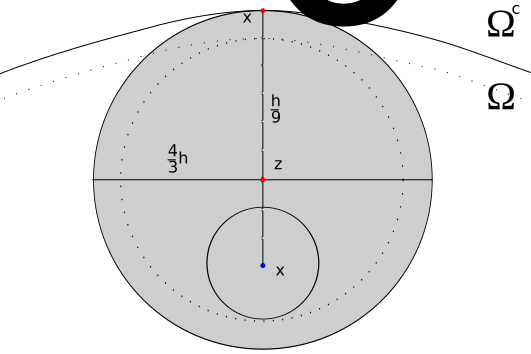
\includegraphics[height=0.55\textwidth, width=0.55\textheight]{Zeichnung1.pdf}
\end{center}
\end{figure}
\end{proof}
There is not a lot to start with if we want to talk about differentiable manifolds. At least it seems like there hasn't been done much in this field by constructive mathematicians. Let's start by defining a simple kind of differentiable manifold. 
\begin{definition} Let $S$ be the unit sphere of the $n$-dimensional euclidean space $\mathbb{R}^n$ and $\phi$ be a homeomorphism. Then $K=\phi(S)$ is called a \textbf{Jordan-manifold}. If additionally $K$ is a $C^1$-manifold with an inside normal function $n:K\rightarrow\mathbb{R}^n$ and a positive real number $r(K)$, such that $\hat{\phi}:B_{r(K)}(S)\rightarrow B_{r(K)}(K)$ defined by $\hat{\phi}(x)=\phi(\frac{x}{|x|})+(1-|x|)n(\phi(\frac{x}{|x|}))$ is a \textbf{$C^k$-Diffeomorphism}, therefore it is $k$-times continuously differentiable with a $k$-times continuously differentiable inverse, then we call $K$ a \textbf{$C^k$-Jordan manifold}.\\
\\
A \textbf{$C^k$-Jordan domain} $\Omega$ is a nonempty bounded open subset of $\mathbb{R}^n$, such that $\partial\Omega$ is a $C^k$-Jordan manifold and for every $x\in\partial\Omega$, $x+\lambda n(x)\in\Omega$ and $x-\lambda n(x)\in\Omega^c$ for all $0<\lambda<r(\partial\Omega)$. Additionally assume that if $x\in\Omega$ and if we can connect $y\in\mathbb{R}^n$ and $x$ by a straight line $s$ that is bounded away from $\partial\Omega$ then $y\in\Omega$.\footnote{Constructive sets can have holes that lack a boundary, therefore this condition is important.}
\end{definition}
\begin{lemma} Let $\Omega$ be a $C^k$-Jordan domain, then $\partial\Omega$ is a $C^k$-submanifold and $\partial\Omega$ coincides with the topological boundary of $\Omega$.
\end{lemma}
\begin{proof}
Let $x\in\partial\Omega$, then since $S$ is a $C^k$-submanifold of $\mathbb{R}^n$ and any $C^k$-parametrization $\psi$ of $S$ around $\phi^{-1}(x)$ can be composed with $\hat{\phi}$ to yield a $C^k$-parametrization of $\partial\Omega$ at $x$.

Denote the topological boundary of $\Omega$ by $K$. It is easy to see that $\partial\Omega\subset K$, for the other inclusion let $x\in K$,  then there exist sequences $(x_n)_{n\geq 0}\subset\Omega$ and $(y_n)_{n\geq 0}\subset\Omega^c$ such that $\lim x_n=\lim y_n=x$. 

The function $\alpha=1-|\hat{\phi}^{-1}|$ yields a positive value for elements of $\Omega$ and a negative value for elements of $\Omega^c$ and is continuous. So we can conclude that $\alpha(x)=0$ since $\alpha(x_n)>h$ and $\alpha(y_n)<h$ for all $n\geq 1$. Therefore $x=\hat{\phi}(\hat{\phi}^{-1}(x))=\phi(\hat{\phi}^{-1}(x))\in\partial\Omega$.
\end{proof}
\begin{definition} Let $\Omega$ be $C^k$-Jordan domain then the function. Then the function $\eta: B_{r(\partial\Omega)}(\partial\Omega)\rightarrow \partial\Omega$ defined by $\eta(x)=\phi(\frac{\hat{\phi}^{-1}(x)}{|\hat{\phi}^{-1}(x)|})$ for $x\in B_{r(\partial\Omega)}(\partial\Omega)$ is called the \textbf{surface projection}.\end{definition}
\begin{lemma} Let $\Omega$ be a $C^k$-Jordan domain ($k>1$), then $\Omega$ is coherent, totally bounded and colocated.
\end{lemma}
\begin{proof} Let $x\in\mathbb{R}^n$, then construct the real number $|x-\Omega^c|$:
Let $n$ be a positive integer then if $|x-\partial\Omega|<\frac{1}{n}$ choose $|x-\Omega^c|_n=\frac{1}{n}$, on the other hand if $|x-\partial\Omega|>\frac{1}{n+1}$ choose $\min(r(\partial\Omega),\frac{1}{n+1})>\epsilon>0$ and $y\in B_{|x-\partial\Omega|-\frac{\epsilon}{2}}(x)$ such that $\frac{\epsilon}{2}<|y-\eta(y)|<\epsilon$ (see Figure 3.2).
\begin{figure}[H]
\begin{center}
\caption{}
	 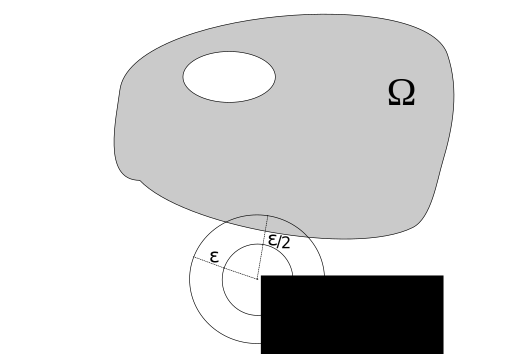
\includegraphics[height=0.55\textwidth, width=0.55\textheight]{Zeichnung.pdf}
\end{center}
\end{figure}
Then, since $y-\eta(y)$ is perpendicular to the tangent space of $\partial\Omega$ at $\eta(y)$ $y-\eta(y)$ and $n(\eta(y))$ are parallel and $\langle n(\eta(y)), y-\eta(y)\rangle$ is either bigger than $-\frac{\epsilon}{4}$ or smaller than $\frac{\epsilon}{4}$. In the former case $x$ is outside of $\Omega^c$ and therefore we have to choose $|x-\Omega^c|_k=|x-\partial\Omega|$ for all $k\geq n$ and in the latter case $x$ is inside of $\Omega^c$ and therefore we choose $|x-\Omega^c|_k=0$ for all $k\geq n$. It's not hard to see that $|x-\Omega^c|$ is a real number. Later in this proof the coherence will imply that in the former case $x$ is indeed in $\Omega$.

We have not yet shown that $\Omega$ is colocated, since we have not given a sequence $(x_n)_{n\geq 0}\subset\Omega^c$ such that $|x-x_n|\rightarrow |x-\Omega^c|$, we have only shown that there is a sequence $(s_n)_{n\geq 0}$ in $\partial\Omega$ such that $|s_n-x|\rightarrow |x-\partial\Omega|$. By the twin tangent ball condition we can just modify $(s_n)_{n\geq 0}$ according to the construction of $|x-\Omega^c|$ and therefore we have to consider the three cases we encountered.\\
In the first case choose $x_n=s_n-\min(r(\partial\Omega),\frac{1}{2n})n(s_n)$, in the second case choose $x_k=s_n-\min(r(\partial\Omega),\frac{1}{2k})n(s_k)$ for all $k\geq n$ and in the third case choose $x_k=x$ for all $k\geq n$.\\
%This remaining property follows if we additionally assume that for all $z\in\partial\Omega$ there exists a $q_z$ such that for all $0<\lambda<q_z$ $z-\lambda n(x)\in\Omega^c$.\\
%The proof of this goes as follows: Since we already have a sequence $(s_n)_{n\geq 0}$ in $\partial\Omega$ such that $|s_n-x|\rightarrow |x-\partial\Omega|$, we just have to modify it according to the construction of $|x-\Omega^c|$ and therefore we have to consider the three cases we encountered. In the first case choose $x_n=s_n-\min(q_{s_n},\frac{1}{2n})n(s_n)$, in the second case choose $x_k=x$ for all $k\geq n$ and in the third case choose $x_k=s_n-\min(q_{s_k},\frac{1}{2k})n(s_k)$ for all $k\geq n$.\\
%Another possibility would be to assume that for each $x\in\partial\Omega$ and each positive $\epsilon$ there exists an element $z\in\Omega^c$ in $B_\epsilon(x)$.
By the same argument one can show that $\Omega$ is located, therefore since $\Omega\subset B_R(0)$ for some positive $R>0$, we can conclude by Proposition 4.5 \cite[p. 95]{CANA} that $\Omega$ is totally bounded.\\
Now we show that $\Omega$ is coherent: Let $x\in\mathbb{R}^n$ be such that $|x-\Omega^c|>0$ then the ball $B_{|x-\Omega^c|-\frac{r(\partial\Omega)}{2}}(x)$ contains an element 
\\$y\in\left\{z\in\mathbb{R}^n:0<|z-\Omega^c|<r(\partial\Omega)\right\}$. The definition of a Jordan domain implies, that we can write $y=\eta(y)+\lambda n(\eta(y))$ for some constant $\lambda$. From our assumption we can conclude, that $\lambda>0$ since we can decide whether $\lambda>0$ or $\lambda<0$ because $|\lambda|>0$ and $\lambda<0$ would imply $|y-\Omega^c|=0$.
Therefore $y\in \Omega$ by definition and as a consequence of that and again the definition of a Jordan domain $x\in\Omega$.

%\\
%\\
%Theorem 4.9 in \cite{CANA}[p. 98] shows that there exists a $\frac{q}{2}<t<q$ such that $\left\{x\in\Omega:|x-\partial\Omega|\geq t\right\}$ is compact and there exists a $t<\hat{t}<q$ %such that $\left\{x\in\Omega:|x-\partial\Omega|<\hat{t}\right\}$ is totally bounded. The compactness of the last set can also be shown using the uniform continuous function $S$ from %lemma 4.9.\\

\end{proof}
\begin{proposition} Let $\Omega$ be a $C^k$-Jordan domain ($k\geq 1$) that admits the twin-tangent ball condition, then for each $x\in B_{r(\partial\Omega)}(\partial\Omega)$ with $|x-\partial\Omega|>0$:
\begin{equation}|\eta(x)-x|=|x-\partial\Omega|\text{ and } |x-z|>|x-\partial\Omega|\end{equation}
for each $z\in \partial\Omega$.
\end{proposition}
\begin{proof}
Let $x\in B_{r(\partial\Omega)}(\partial\Omega)$. Then obviously $|x-\eta(x)|\geq |x-\partial\Omega|$ and lemma 3.13 enables us to decide whether $x\in\Omega$ or $x\in\Omega^c$.\\
Without loss of generality assume $x\in\Omega$ and observe that $M_+(\eta(x))-\eta(x)$ as well as $x-\eta(x)$ are perpendicular to the tangent space of $\partial\Omega$ at $\eta(x)$. Therefore $B_{|x-\partial\Omega|}(x)\subset B_{r(\partial\Omega)}(M_+(x))\subset\Omega$, which immediately implies the desired result.
\end{proof}
\begin{lemma} Let $\Omega$ be a $C^k$-Jordan domain ($k\geq 1$), admitting the twin tangent ball condition, then the open subset $\Omega_h=\left\{x\in\Omega: |x-\Omega^c|>h\right\}$ for $0<h<r(\partial\Omega)$ is a $C^k$ Jordan domain, admitting a twin tangent ball condition.\end{lemma}
\begin{proof} 
First of all set $\phi_{\partial\Omega_h}=\phi+hn\circ\phi$, which is a homeomorphism with inverse $\phi_{\partial\Omega_h}^{-1}=\phi^{-1}\circ\eta$. If we choose $r(\partial\Omega_h)=r(\partial\Omega)-h$ and $n_{\partial\Omega_h}=n\circ\eta$ we get for every $x\in B_{r(\partial\Omega_h)}(S)$ that
\begin{equation*}\hat{\phi}_{\partial\Omega_h}(x)=\phi_{\partial\Omega_h}(\frac{x}{|x|}) +(1-|x|)n_{\partial\Omega_h}(\phi_{\partial\Omega_h}(\frac{x}{|x|}))=\hat{\phi}(x)+hn(\phi(\frac{x}{|x|}))\end{equation*}
which shows that $\hat{\phi}_{\partial\Omega_h}:B_{r(\partial\Omega_h)}(S)\rightarrow B_{r(\partial\Omega_h)}(\partial\Omega_h)$ is a $C^k$-Diffeomorphism and we conclude that $\Omega_h$ is a $C^k$-Jordan domain.

We can choose $r(\Omega_h)$ such that for each $x\in\partial\Omega_h$ the ball $B_{r(\Omega_h)}(x+r(\Omega_h)n(x))$ is contained in $\Omega_h$ and the ball $B_{r(\Omega_h)}(x-r(\Omega_h)n(x))$ is contained in $\Omega_h^c$: 
Let $x\in\partial\Omega_h$, $r_0=\min(h,\frac{r(\partial\Omega)-h}{2})$ and $y_\pm\in B_{r_0}(x\pm r_0n(\eta(x)))$ then if we assume that $|y_+-\eta(y_+)|<h$ we get that:
\begin{align*}r_0+h&=|x+r_0n(\eta(x))-\eta(x)|\\
&<|x+r_0n(\eta(x))-\eta(y_+)|\\
&\leq |x+r_0n(\eta(x))-y_+|+|y_+-\eta(y_+)|\\
&< r_0+h\end{align*}
which is a contradiction, therefore $|y_+-\eta(y_+)|\geq h$ and if we choose $r(\Omega_h)$ slightly smaller than $r_0$ the corresponding ball is inside $\Omega_h$.

If we assume $|y_--\eta(y_-)|>h$ we get an analogous contradiction:
\begin{align*} h<|y_--\eta(y_-)|&<|y_--\eta(x)|\\
&\leq|y_--(x-r_0n(\eta(x)))|+|x-r_0n(\eta(x))-\eta(x)|\\
&<r_0+ (h-r_0)=h\end{align*}

and therefore $\Omega_h$ admits the twin tangent ball condition.
\end{proof}

%Finally we can prove that $C^k$-Jordan domains ($k\geq 1$) admit the constriction property. %The idea behind the construction of the constriction functions $\phi_\epsilon$ is just to use the part of $\Omega$ that behaves like $\partial\Omega\times(0,h)$ for $h>0$ and exploit this property, because it is pretty straight forward to constrict $\partial\Omega\times(0,h)$ into itself.
\begin{theorem} Let $\Omega$ be a $C^k$-Jordan domain ($k\geq 1$) then $\Omega$ admits the constriction property.
\end{theorem}
\begin{proof}
Let $\min(1,\frac{r(\partial\Omega)}{2})>h>0$ and $\frac{h}{2}>\epsilon>0$. We first define a diffeomorphism $f_\epsilon:\left\{x\in\mathbb{R}^n:1-h<|x|<1-\nu\right\}\rightarrow\left\{x\in\mathbb{R}^n:1-h<|x|<1\right\}$, such that $U=\left\{x\in\mathbb{R}^n: 1-h<|x|<1-\frac{h}{2}\right\}$ is invariant under $f_\epsilon$, where $\nu$ is a positive real number that will be chosen later:\\
Let $g:[0.h]\rightarrow [1-\frac{\nu}{2},1]$ be a monotone continuously differentiable map that restricted to $(0,\frac{h}{2})$ is $1$, $g(h)=1-\frac{\nu}{2}$ and $g\prime\leq\nu$  then define 
\begin{equation*}f_\epsilon(x)=(1-h)\frac{x}{|x|}+(|x|-(1-h))g(|x|-1+h)\frac{x}{|x|}\end{equation*}
which is continuously differentiable and has a continuously differentiable inverse and leaves $U$ invariant. We can calculate the differential $Df_\epsilon$:
\begin{align*}Df_\epsilon(x)&=(\frac{1-h}{|x|}+(1-\frac{1-h}{|x|})g(|x|-1+h))Id\\
&+\frac{(1-h)(g(|x|-1+h)-1)}{|x|}A\\
&+(|x|-(1-h))g\prime(|x|-1+h)A\\\end{align*}
where the matrix $A$ is defined by:
\begin{equation*}A=\begin{bmatrix}
\frac{x_1^2}{|x|^2}	& \frac{x_1x_2}{|x|^2}	& \dots	 & \frac{x_1x_n}{|x|^2}    \\
\frac{x_2x_1}{|x|^2}	& \frac{x_2^2}{|x|^2} 	& \dots  & \frac{x_2x_n}{|x|^2} 	  \\
\vdots	& \vdots  	& \ddots & \vdots \\
\frac{x_nx_1}{|x|^2} 	& \dots & \frac{x_nx_{n-1}}{|x|^2}	 & \frac{x_n^2}{|x|^2}
\end{bmatrix}\end{equation*}
At this point we define $A_\epsilon=\left\{x\in\Omega: |x-\Omega^c|>\nu\right\}$ and $\psi_\epsilon$ by transporting the function $f_\epsilon$ on $A_\epsilon$ by setting $\psi_\epsilon=\hat{\phi}\circ f_\epsilon\circ\hat{\phi}^{-1}$ on $\left\{z\in A_\epsilon: |z-\Omega^c|<h\right\}$ and by setting it equal to the identity on $\left\{x\in\Omega: |x-\Omega^c|>h\right\}$.\\ We can extend by continuity using lemma 3.7 in \cite[p. 91]{CANA} on the whole $A_\epsilon$ since we have already defined the function on a located subset and its metric compliment in $A_\epsilon$ and therefore on a dense subset of $A_\epsilon$.\\
We get immediately that this is a diffeomorphism and that since:
\begin{equation*}|f_\epsilon(x)-x|<\frac{\nu}{2}\end{equation*}
for each $x\in\left\{x\in\mathbb{R}^n: 1-h<|x|<1-\nu\right\}$, if we choose $\nu<2\omega(\epsilon)$, where $\omega$ is the modulus of continuity of $\hat{\phi}$, we get for each $z\in A_\epsilon$:
\begin{equation*}|\psi_\epsilon(z)-z|<\epsilon\end{equation*}
Next we show that $|Id-D\psi_\epsilon|_\infty<\epsilon$:
\begin{align*} |Id-D\psi_\epsilon|_\infty&=|Id-D\hat{\phi}\circ Df_\epsilon\circ D\hat{\phi}^{-1}|_\infty\\
&\leq|D\hat{\phi}|_\infty|D\hat{\phi}^{-1}|_\infty|Id- Df_\epsilon|_\infty\\
\end{align*} 
We get the following estimate for the last factor, using the properties of $g$ to get our desired estimates:
\begin{align*} |Id- Df_\epsilon|_\infty&\leq\underset{<\nu}{\underbrace{|1-(\frac{1-h}{|x|}+(1-\frac{1-h}{|x|})g(|x|-1+h))|}}\\
&+\underset{<\nu}{\underbrace{|\frac{(1-h)(g(|x|-1+h)-1)}{|x|}|}}|A|_\infty\\&+\underset{<h\nu}{\underbrace{|(|x|-(1-h))g\prime(|x|-1+h)}}|A|_\infty\\
\end{align*}
If we choose $\nu<\epsilon\min(1,\inf_{x\in B_h(S)}\frac{1}{|D\hat{\phi}|_\infty|D\hat{\phi}^{-1}|_\infty(1+(1+h)|A|_\infty)}(x))$\footnote{The infimum exists, since $D\hat{\phi}$ and $D\hat{\phi}^{-1}$ are uniformly continuous by assumption on every compact subset of $B_{r(\partial\Omega)}(\partial\Omega)$.} we get the desired result.


It remains to show that the family $(A_\epsilon)_{h>\epsilon>0}$ of subsets of $\Omega$  has the properties we want it to have:
By lemma 3.12 we get that they are $C^k$-Jordan domains admitting the twin tangent ball condition, which together with lemma 3.11 implies that they are colocated, totally bounded and coherent. The integrability of $\Omega$ and $A_\epsilon$ follows since we can using substitution estimate:

\begin{align*}\int_{\Omega\setminus A_\epsilon} 1\mathrm{d}\lambda&=\int_{\hat{\phi}(\left\{1-\nu<|x|<1\right\})} 1\mathrm{d}\lambda=\int_{(\left\{1-\nu<|x|<1\right\}} |\det\hat{\phi}|d\lambda\\
&\leq C_n\nu\sup_{x\in B_h(S)}|\det\hat{\phi}|<\epsilon\end{align*}
The last term can be chosen small enough if we additionally choose $\nu<(C_n\sup_{x\in B_h(S)}|\det\hat{\phi}|)^{-1}$, where $C_n$ is a real number only dependent on the dimension of the domain $\Omega$.\\
The family of subsets $(A_\epsilon)_{\epsilon>0}$ together with the family $(\psi_\epsilon)_{\epsilon>0}$ of diffeomorphisms fulfill the requirements of the constriction property for $\Omega$.



%Let $h<\min(r(\partial\Omega),\underset{x\in\partial\Omega}{\sup}|Dn(x)|)$, $\epsilon$ be a positive real number and \\$\nu=\epsilon\min(\frac{1}{h},\frac{1}{|\partial\Omega|},\frac{1}{\underset{x\in\Omega}{\sup}|id-(D\omega(x)+hDn(\omega(x))|})$, then define the function $\phi_\epsilon^{-1}$ by
%\begin{small}
%\begin{align*}\phi_\epsilon^{-1}(x)&=\omega(x)+hn(\omega(x))-\langle x-(\omega(x)+hn(\omega(x))),n(\omega(x))\rangle n(\omega(x))(1-\nu)\\
%&=x-\nu(x-(\omega(x)+hn(\omega(x))))
%\end{align*} 
%\end{small}
%\begin{figure}[H]
%\begin{center}
%	 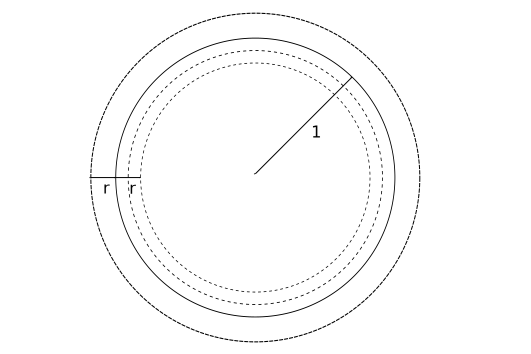
\includegraphics[height=0.5\textwidth, width=0.5\textheight]{Zeichnung3.pdf}
%\end{center}
%\end{figure}
%on the subset $C=\left\{x\in\Omega: |x-\Omega^c|<h\right\}$ and $\phi_\epsilon^{-1}(x)=x$ for $x\in C^c$. \\
%\\
%$C$ is located in $\Omega$, therefore $C\cup C^c$ is dense in $\Omega$, and since $\phi_\epsilon$ is uniformly continuous on $C\cup C^c$ there exists an extension, by abuse of notation also denoted by $\phi_\epsilon$, on the whole $\Omega$. \\
%\\
%Choose $\hat{C}=C\cup C^c$.\\
%\\
%Furthermore define the correspoinding compact exhaustion $(A_\epsilon)_{\epsilon>0}$ by 
%\begin{equation*}A_\epsilon=\left\{x\in\Omega: |x-\Omega^c|>\nu\right\}\end{equation*} 

%$A_\epsilon$ is a $C^1$-boundary by Lemma 3.10 and by Proposition 3.3 has the desired properties.\\
%\\
%The sets $\Omega$, $C$ and $A_\epsilon$ are integrable, since they have a continuous boundary and $|\Omega\setminus A_\epsilon|\leq \nu|\partial\Omega|\leq\epsilon$: \\
%\\
%If necessary choose $\nu$ small enough such that $|\det{DS}||\partial\Omega|<\epsilon$, which is possible since the determinant is continuous, and we can see that it is sufficient since:
%\begin{equation*}\int_{A_\epsilon}1d\lambda=\int_{S(\partial\Omega\times(0,\nu))}1d\lambda=\int_{\partial\Omega\times(0,\nu)}|\det{DS}|d\lambda\end{equation*}
%Let $x\in\Omega$ then
%\begin{align*}
%|\phi_\epsilon(x)-x|\overset{y=\phi_\epsilon^{-1}(x)}{=}|y-\phi_{\epsilon}^{-1}(y)|&=\nu|x-(\omega(x)+hn(\omega(x)))|\\
%&\leq\nu h<\epsilon
%\end{align*}
%Lemma 3.9 and the fact that $\Omega$ has a $C^2$-boundary the functions, implies that $\phi_\epsilon^{-1}$ is differentiable on $C$ and $C^c$. Therefore one can write down their Differentials:
%\begin{equation*}D\phi_{\epsilon}^{-1}(x)=Id-\nu(Id-(D\omega(x)+hDn(\omega(x))))\end{equation*}
%It remains to examine the term $Id-(D\omega(x)+hDn(\omega(x)))$. \\First the differential of $\omega$ can be derived by starting with the construction of lemma 3.9.\\
%Let $x\in(0,1)^{n-1}$ and $s\in (0,h)$ then
%\begin{equation*}DS(x,s)=\begin{pmatrix}D\psi+(Dn\circ\phi)s& \begin{matrix}0\\n\circ\psi\end{matrix}\end{pmatrix}\end{equation*}
%and since $\phi^{-1}\circ\omega$ equals the projection onto the first $n-1$ coordinates of $S^{-1}$ we infer that 
%\begin{equation*}D\omega(x)=(Id+Dn(\omega(x))|x-\Omega^c|)^{-1}\end{equation*}
%This inverse can be computed using the geometric series technique and it can be shown to be uniformly continuous for $|x-\Omega^c|<h$. Therefore we get that
%\begin{align*} |Id-D\phi_\epsilon^{-1}(x)|\leq \nu\text{ }\underset{x\in C}{\sup}|id-(D\omega(x)+hDn(\omega(x))\circ D\omega(x)|<\epsilon\end{align*}
\end{proof}
\begin{theorem} Let $\Omega$ be a totally bounded, coherent, colocated and star-shaped domain then $\Omega$ admits the constriction property.
\end{theorem}
\begin{proof} Let $x_0\in\Omega$ a center of $\Omega$, $\epsilon>0$ and $R$ be a bound of $\Omega-x_0$. If we define our diffeomorphisms by $\phi_\epsilon^{-1}(x)=x_0+(1-\frac{\epsilon}{R})(x-x_0)$, and our internally approximating family of subsets of $\Omega$ by $A_\epsilon=\phi_\epsilon^{-1}(\Omega)$, we immediately get our desired properties, since $\phi_\epsilon$ is only translating and scaling.
\end{proof}
The initial plan was to show the constriction property for piecewise linearly bounded domains, but all attempts became very technical, and I decided to define a nice class of domains for whom the construction goes pretty easy and whose properties I suspect are admitted by a big class of familiar domains. 
\\
The proof of Theorem 3.11 can of course be extended to domains, whose boundary is the union of finitely many well separated $C^k$-Jordan manifolds ($k>1$). 
\section{Open problems}
There are a few questions that I couldn't answer in this thesis because at some point I felt that I had to stop, since every time I answered a question more questions arose. So here are some of the questions I would like to answer or to have answered:
\begin{enumerate}
\item{Do surface projections exist for general $C^1$-domains, admitting a twin tangent ball condition?}
\item{Is every manifold that is $C^{k+1}$-diffeomorphic to the sphere a $C^k$-Jordan manifold?}
\item{Does every $C^1$-Jordan manifold admit the twin tangent ball condition?}
\end{enumerate}

%In my personal opinion a "'practical constructive domain"' $\Omega$ should admit the following properties. It should be located as well as colocated and there should be a methods that allows you to decide for an arbitrary $x\in\mathbb{R}^n$ and $\epsilon>0$ whether $x$ is in $\Omega$, in the metric complement of $\Omega$ or in $B_\epsilon(\partial\Omega)$. The latter means that $\Omega$ and $\Omega^c$ should be coherent. The first condition automatically implies that $\partial\Omega$ is non-empty. Given that $\Omega$ and its metric complement are coherent we can prove that locatedness \& colocatedness is equivalent to the locatedness of the boundary. \\
%Strong integrability of the boundary provides a sufficient condition for the existence of an internal approximation by compact sets


\chapter{Rellich Compactness}
This chapter is devoted to the Rellich-Kondrachov Theorem, which states the total boundedness of the $H^1_0(\Omega)$-unit-ball with respect to the $L^2(\Omega)$-norm under certain assumptions on the boundary. As mentioned in the chapter "The constructive Dirichlet problem" Michael(Yuchuan) Wang has shown in his doctoral thesis \cite{Wang} that this statement is equivalent to the existence of solutions of the Dirichlet problem for arbitrary $L^2$-functions as an inhomogeneity.\\
The main result of this chapter is the proof of this theorem for bounded domains that admit the constriction property and a family of arbitrary fine meshes. The proof is mainly inspired by the one found in Prof. Haslinger's lecture notes \cite{Haslinger}. Although a lot of the details have changed the main idea of using a mollifier and then proving the total boundedness for the set of mollified functions remained.\\
\\
The main differences lie in the final step where in the original proof Arzel\'{a}-Ascoli's theorem is used to show the existence of an $\epsilon$-approximation of the set of mollified elements of $B_{H^1_0}$. 

First of all the application of Arzel\'{a}-Ascoli's theorem has constructively much stronger requirements, than in the classical case that are not as obviously fulfilled and secondly we wouldn't get an $\epsilon$-approximation within $B_{H^1_0}$ since the method provides no tool to control the $H^1_0(\Omega)$-norm and fix the boundary condition. The reason for this additional properties will be discussed in the Appendix.
\\
\\
The structure of the proof is as follows: In order to prove some estimates involving mollification, the functions are extended on the whole $\mathbb{R}^n$ to circumvent any possible problem with this approach. After we established that we can control the $L^2(\Omega)$-norm as well as the $H^1_0(\Omega)$-norm of the mollified functions and of their interpolations we use the functions $\phi_\epsilon$
as pullbacks and prove that we can control the $L^2(\Omega)$-norm and $H^1_0(\Omega)$-norm of the pulled back functions. Now that we are on $A_\epsilon$ we can mollify such that the boundary condition does not get violated and we keep the $H^1_0(\Omega)$-norm under our control. Interpolation, multiplication by a constant close to one and the total boundedness of balls in finite dimensional normed-vector-spaces (Theorem 1.16) yields the final result.
\\
\\
As a preparation of the proof a few lemmas are necessary.
\begin{lemma} Let $\Omega$ be a colocated and coherent domain, then for each $f\in C^1_0(\Omega)$ there is a function $F\in C^1_0(\mathbb{R}^n)$ extending $f$ on the whole space by $0$ i.e: $F|_\Omega=f$, $F|_{\Omega^c}=0$.\end{lemma}
\begin{proof} Let $f\in C^1_0(\Omega)$, therefore there exists a compact support $D$ of $f$ and $\delta(D)>0$, such that $B_{\delta(D)}(D)\subset \Omega$, and let $y\in\mathbb{R}^n$. Then either $|y-\Omega^c|>0$ or $|y-\Omega^c|<\delta(D)$. In the former case it follows since $\Omega$ is coherent that $y\in\Omega$ and we can set $F(y)=f(y)$. In the latter case $y\in D^c$ and we can set $F(y)=0$. Therefore $F$ is a function on $\mathbb{R}^n$ and $F$ is obviously continuously differentiable.
\end{proof}
In the following lemmas we will use lemma 4.1 implicitly:
\begin{lemma} Let $\Omega$ be as in lemma 4.1 and $u\in C^1_0(\Omega)$ then \begin{small}\begin{equation}||u(.+h)-u||_{L^2(\mathbb{R}^n)}\leq|h|||u||_{H^1_0(\Omega)}\end{equation}\end{small}\end{lemma}
\begin{proof}\cite{Haslinger}[p. 35]: Let $x\in\Omega$ and $h\in\mathbb{R}^n$. Starting at the fundamental theorem of calculus:
\begin{equation*} u(x+h)-u(x)=\int_0^1\nabla u(x+th)h\mathrm{d}t\end{equation*}
Integrating the square of the expression and estimating yield the result:
\begin{align*}
\int_{\mathbb{R}^n}|u(x+h)-u(x)|^2\mathrm{d}\lambda(x)&\overset{\text{Jensen}}{\leq} |h|^2\int_{\mathbb{R}^n}\int_0^1|\nabla u(x+th)|^2\mathrm{d}t\mathrm{d}\lambda(x)\\
&\overset{\text{Fubini}}{=}|h|^2\int_0^1\int_{\mathbb{R}^n}|\nabla u(x+th)|^2\mathrm{d}\lambda(x)\mathrm{d}t\\
&=|h|^2||u||_{H^1_0(\Omega)}^2
\end{align*}
\end{proof}
\begin{remark}By a similar argument one can prove the Poincar\'{e} inequality \\$||u-\frac{1}{|\Omega|}\int_\Omega u\mathrm{d}\lambda||_{L^2(\Omega)}\leq 2R||u||_{H^1_0(\Omega)}$ for domains contained in a ball of radius $R$.\end{remark}
Using (3.2) of the definition of the constriction property, we can show a similar result:
\begin{lemma}Let $\Omega$ be a domain satisfying the constriction property, $h>0$ and $u\in H^1_0(\Omega)$ and $h>0$. Then the following estimate holds true:
\begin{equation}\int_{A_h}|u(\phi_h(x))-u(x)|^2d\lambda(x)\leq h^2(1+\gamma(h))||u||_{H^1_0(\Omega)}^2\end{equation}
\end{lemma}
\begin{proof}
Let $u\in H^1_0(\Omega)$ and $h>0$. We again start at the fundamental theorem of calculus:
\begin{equation*} u(\phi_h(x))-u(x)=\int_0^1\nabla u(x+t(\phi_h(x)-x))(\phi_h(x)-x)\mathrm{d}t\end{equation*}
Just as in the previous lemma we use Jensen's inequality and Fubini's theorem:
\begin{small}
\begin{align*}&\int_{A_h}|u(\phi_h(x))-u(x)|^2d\lambda(x)\\& \leq \int_0^1\int_{A_h}|\nabla u(x+t(\phi_h(x)-x))|^2|(\phi_h(x)-x)|^2d\lambda(x)dt\end{align*}
Now we use (3.1) of the definition of the constriction property:
\begin{align*}\leq h^2\int_0^1\int_{A_h}|\nabla u(x+t(\phi_h(x)-x))|^2d\lambda(x)dt\end{align*}
Next we expand by $|det(Id+t(D\phi_h(x)-Id))|$ and used the fact that $|det(Id+t(D\phi_h(x)-Id))|^{-1}<1+\gamma(h)$.
\begin{align*}\leq h^2(1+\gamma(h))\int_0^1\int_{A_h}\nabla u(x+t(\phi_h(x)-x))|^2|det(Id+t(D\phi_h(x)-Id))|d\lambda(x)dt\end{align*}
Finally we can use substitution, since the map $x\mapsto x+t(\phi_h(x)-x)$ is injective as a consequence of (3.2) in the definition of the constriction property.
\begin{align*}\leq h^2(1+\gamma(h))\int_0^1\int_{\Omega}|\nabla u(x)|^2d\lambda(x)dt=h^2(1+\gamma(h))||u||_{H^1_0(\Omega)}^2
\end{align*}
\end{small}
\end{proof}

\begin{definition} Let $\chi\in C^1_0(\mathbb{R}^n)$, such that $\chi\geq 0$, $\int_{\mathbb{R}^n}\chi d\lambda=1$ and $\chi|_{\mathbb{R}^n\setminus B_{\mathbb{R}^n}}=0$. Then  we call the family of functions $(\chi_\delta)_{\delta>0}$ defined for each $\delta>0$ and each $x\in\mathbb{R}^n$ by 
$\chi_\delta(x)=\frac{\chi(\frac{x}{\delta})}{\delta^n}$
a \textbf{mollifier}. \end{definition}
\begin{lemma} Let $\Omega$ be as in lemma 4.1, $\delta>0$, $\chi_\delta$ be a mollifier and $u\in C^1_0(\Omega)$ then \begin{small}\begin{equation}||\chi_\delta*u-u||_{L^2(\mathbb{R}^n)}\leq\delta||u||_{H^1_0(\Omega)}\end{equation}\end{small}\end{lemma}
\begin{proof}\cite{Haslinger} [p. 29-35] : Let $u\in C^1_0(\Omega)$
\begin{align*}||\chi_\delta*u-u||_{L^2(\mathbb{R}^n)}^2&=\int_{\mathbb{R}^n}(\int_{\mathbb{R}^n}\chi_\delta(x-y)(u(y)-u(x))\mathrm{d}\lambda(y))^2\mathrm{d}\lambda(x)\\
&\overset{\text{Jensen}}{\leq} \int_{\mathbb{R}^n}\int_{\mathbb{R}^n}\chi_\delta(x-y)(u(y)-u(x))^2\mathrm{d}\lambda(y)\mathrm{d}\lambda(x)\\
&\overset{\text{Subst. \& Fubini}}{=} \int_{\mathbb{R}^n}\chi_\delta(y)\int_{\mathbb{R}^n}(u(x-y)-u(x))^2\mathrm{d}\lambda(x)\mathrm{d}\lambda(y)\\
&\overset{\text{Lemma 4.2 }}{=} \int_{\mathbb{R}^n}\chi_\delta(y)|y|^2||u||_{H^1_0(\Omega)}^2\mathrm{d}\lambda(y)\leq \delta^2||u||_{H^1_0(\Omega)}^2\end{align*}
\end{proof} 
\begin{remark} Let $\Omega$ be a colocated domain, then $B_\delta(\Omega)$, where $\delta>0$, is not necessarily colocated. \\It is easy to construct a Brouwerian counterexample, such that if the former statement is provable, LPO would hold: Take for example an annulus $A$ with inner radius $r$. If $B_\delta(A)$ would be colocated for all $\delta>0$ we would have a method to decide whether $\delta\leq r$ or $\delta> r$.\end{remark}
\begin{lemma} Let $\Omega$ and $\chi_\delta$ be as in lemma 4.1, then for any $u\in C^1_0(\Omega)$ the following estimate holds true:
\begin{small}\begin{equation}||\chi_\delta*u||_{H^1_0(\mathbb{R}^n)}\leq||u||_{H^1_0(\Omega)}\end{equation}\end{small}\end{lemma}
\begin{proof} Let $u\in C^1_0(\Omega)$
\begin{align*}||\chi_\delta*u||_{H^1_0(\mathbb{R}^n)}^2&=\int_{\mathbb{R}^n}(\nabla_x \int_{\mathbb{R}^n}\chi_\delta(x-y)u(y)\mathrm{d}\lambda(y))^2\mathrm{d}\lambda(x)\\
&\overset{\text{Subst.}}{=}\int_{\mathbb{R}^n}(\int_{\mathbb{R}^n}\chi_\delta(y)\nabla_x u(x-y)\mathrm{d}\lambda(y))^2\mathrm{d}\lambda(x)\\
&\overset{\text{Subst.}}{=}\int_{\mathbb{R}^n}(\int_{\mathbb{R}^n}\chi_\delta(x-y)\nabla_y u(y)\mathrm{d}\lambda(y))^2\mathrm{d}\lambda(x)\\
&\overset{\text{Jensen}}{\leq}\int_{\mathbb{R}^n}\int_{\mathbb{R}^n}\chi_\delta(x-y)(\nabla u(y))^2\mathrm{d}\lambda(y)\mathrm{d}\lambda(x)\\
&\overset{\text{Fubini}}{=}\int_{\mathbb{R}^n}\int_{B_\delta(\Omega)}\chi_\delta(x-y)\mathrm{d}\lambda(x)(\nabla u(y))^2\mathrm{d}\lambda(y)\\
&=\int_{\mathbb{R}^n}(\nabla u(y))^2\mathrm{d}\lambda(y)=||u||_{H^1_0(\Omega)}^2\end{align*}
\end{proof}
\begin{definition} Let $C_h$ be a mesh of a domain $\Omega$ with meshsize $h$. Then the interpolation operator corresponding to the mesh is given by $I_h(u)=\sum_{i=1}^{M_h}u(x_i)\phi_i$ for $u\in C(\Omega)$, where $\phi_i$ are the Lagrangian-shape-functions.\end{definition}
\begin{remark} The Lagrangian-shape-functions on $\Omega$ corresponding to the mesh $C_h$ can be constructed on $\Omega\cap\mathbb{Q}$ the same way as in the classical case and then extended on the whole $\Omega$ by Lemma 3.7 in \cite[p. 91]{CANA}.
\end{remark}
\begin{lemma} Let $\Omega$ be an open subset of $\mathbb{R}^n$, with a corresponding mesh $C_h$ of meshsize $h>0$, $\epsilon>0$ and $f\in C^1(\Omega)$. Denote the modulus of continuity of $\nabla f$ by $\omega$. Then if $h<\omega(\epsilon)$, $|\nabla(I_h(f)-f)|_2<\epsilon$\footnote{Where $|.|_2$ is the standard euclidean norm on $\mathbb{R}^n$.}.\end{lemma}
\begin{proof} Let $\epsilon>0$, $\nu>0$ a constant to be chosen later in this proof and $h<\omega(\nu)$.
Start at an arbitrary element $K$ of the mesh and without loss of generality assume that it is a right simplex.\\
Let $x_0$ be the vertex of $K$ adjacent to the right-angle, $x_k$ be an arbitrary vertex of $K$ distinct from $x_0$. The mean-value-theorem yields
\begin{small}\begin{equation*}f(x_k)-f(x_0)=\int_0^1\nabla f(x_0 t+x_k(1-t))(x_k-x_0)dt\end{equation*}\end{small} 
Consider the orthonormal basis $(e_i)_{i=1}^n$ of $\mathbb{R}^n$ defined $e_k=\frac{x_k-x_0}{|x_k-x_0|}$. \\
\\
For each $x\in K$ we get that for the component of $\nabla f(x)$ in the direction $e_k$ the estimate:
\begin{small}\begin{align*}|f(x_k)-f(x_0)-\nabla f(x)(x_k-x_0)|&=|\int_0^1(\nabla f(x)-\nabla f(x_k t+x_0(1-t)))(x_k-x_0)dt|\\&\leq\nu|x_k-x_0|\end{align*}\end{small} 
This immediately implies that for the component of $\nabla I_h(f)$ in the direction $e_k$ on $K$ we get:
\begin{small}\begin{equation*}|\nabla f(x)e_k-\nabla I_h(f)e_k|\leq\nu\end{equation*}\end{small}
which further implies:
\begin{equation*}|\nabla f(x)-\nabla I_h(f)(x)|_2\leq\sqrt{n}\nu\end{equation*} for each $x\in \Omega$. So we get our desired result if we choose $\nu=\frac{\epsilon}{\sqrt{n}}$
\end{proof}

\begin{lemma} Let $\epsilon>0$ and $\Omega$ be as in lemma 4.1, with the additional property that there exists a family of arbitrary fine meshes $(C_q)_{q>0}$ of $\Omega$. \\Furthermore let $A\subset\subset\Omega$ be open, $R>0$ such that $\Omega\subset B_R(0)$ and $\delta>0$ such that $B_\delta(A)\subset\Omega$. 
Then there exists a meshsize $h>0$ admitting the following estimates:
\begin{small}\begin{equation} ||I_h(\chi_\delta*u)-\chi_\delta*u||_{L^2(\Omega)}\leq \epsilon||u||_{H^1_0(\Omega)}\end{equation}\end{small}
\begin{small}\begin{equation} ||I_h(\chi_\delta*u)-\chi_\delta*u||_{H^1_0(\Omega)}\leq \epsilon||u||_{H^1_0(\Omega)}\end{equation}\end{small}
for every $u\in C^1_0(\Omega)$, with a support contained in $A$.
\end{lemma}
\begin{proof}Let $\epsilon>0$, $u\in C^1_0(\Omega)$, with a support contained in $A$, and \\$h<\min(\omega(\frac{\epsilon}{|B_R(0)|C_p}),\hat{\omega}(\frac{\epsilon}{|B_R(0)|C_p}))$, where $\omega$ is the modulus of continuity of $\chi_\delta$, $\widehat{\omega}$ is the modulus of continuity of $\nabla\chi_\delta$ and $C_p$ is the Poincar\'{e} constant of $\Omega$.\\
\\First we estimate using the continuity of $\chi_\delta$ and a little trick to get inequality (4.5):
\begin{small}
\begin{align*}||I_h(\chi_\delta*u)&-\chi_\delta*u||_{L^2(\Omega)}^2=\\
=&\int_{\Omega}((\sum_{i=1}^{M_h}\int_{A}\chi_\delta(x_i-y)u(y)\mathrm{d}\lambda(y)\phi_i(x))-\int_{A}\chi_\delta(x-y)u(y)\mathrm{d}\lambda(y))^2\mathrm{d}\lambda(x)\\
=&\int_{\Omega}(\int_{A}(\sum_{i=1}^{M_h}(\chi_\delta(x_i-y)\phi_i(x))-\chi_\delta(x-y))u(y)\mathrm{d}\lambda(y))^2\mathrm{d}\lambda(x)\\
\overset{\text{pos. \& cont.}}{\leq}&\int_{\Omega}(\int_{A}(\frac{\epsilon}{|B_R(0)|C_p})u(y)\mathrm{d}\lambda(y))^2\mathrm{d}\lambda(x)\\
\overset{\text{Jensen}}{\leq} &\int_{\Omega}1\mathrm{d}\lambda|\Omega|(\frac{\epsilon}{|B_R(0)|C_p})^2||u||_{L^2(\Omega)}^2=\epsilon^2\frac{||u||^2_{L^2(\Omega)}}{C_p^2}\\
\overset{\text{Poincar\'{e}}}{\leq}&\epsilon^2||u||_{H^1_0(\Omega)}^2.
\end{align*}
\end{small}
Second we do as in the previous estimate, but this time use the continuity of $\nabla\chi_\delta$ and lemma 4.11 to arrive at inequality (4.6):
\begin{small}
\begin{align*}
||I_h(\chi_\delta*u)-&\chi_\delta*u||_{H^1_0(B_\delta(\Omega))}^2\\
&=\int_{\Omega}(\int_{A}\nabla_x(\sum_{i=1}^{M_h}(\chi_\delta(x_i-y)\phi_i(x))-\chi_\delta(x-y))u(y)\mathrm{d}\lambda(y))^2\mathrm{d}\lambda(x)\\
&\leq \int_{\Omega}1\mathrm{d}\lambda(x)|\Omega|(\frac{\epsilon}{|B_R(0)|C_p})^2||u||_{L^2(\Omega)}^2=\epsilon^2\frac{||u||^2_{L^2(\Omega)}}{C_p^2}\\
&\leq\epsilon^2||u||_{H^1_0(\Omega)}^2.
\end{align*}
\end{small}
\end{proof}
\begin{lemma} Let $\epsilon>0$, $\Omega$ be as in lemma 4.1 that additionally admits the constriction property. Then for each $h>0$ and $u\in C^1_0(\Omega)$ we get that $u\circ\phi_h\in C^1_0(A_h)$ and \begin{equation} ||u\circ\phi_h||_{H^1_0(\Omega)}^2\leq\frac{(1+h)^2}{1-\gamma(h)}||u||_{H^1_0(\Omega)}^2\end{equation} 
Additionally there exists $q>0$ such that \begin{equation} ||u\circ\phi_q-u||_{L^2(\Omega)}<\epsilon||u||_{H^1_0(\Omega)}\end{equation}
\end{lemma}
\begin{proof}Let $u\in C^1_0(\Omega)$, $h>0$ and $s>0$ such that $B_s(F)\subset\Omega$, where $F$ is a compact support of $u$. The constriction property entails the total boundedness of $\Omega$ and therefore we can assume that there is a $R>0$ such that $\Omega\subset B_R(0)$. The set $C=\left\{x\in\Omega:|x-\Omega^c|\leq\frac{s}{2}\right\}$ is totally bounded by \cite[Theorem 4.9 p.98]{CANA} since $\Omega$ is totally bounded  and $|x-\Omega^c|$ is uniformly continuous. Obviously the distance between $C$ and $F$ is bigger than $\frac{s}{2}$.\\
$\phi_h^{-1}$ is hyperinjective by Proposition 3.2 and therefore there is an $r>0$ such that the images of $F$ and $C$ under $\phi_h^{-1}$ are a distance of $r$ apart from each other. By Proposition 3.2 the extension of $\phi_h$ on $\overline{\Omega}$ maps $\partial A_h$ onto $\partial \Omega$. Therefore every ball with origin in $A_h$ that intersects $A_h^c$ contains a point of $\phi_h^{-1}(C)$. As a result we get that for any given point $x\in\phi_h^{-1}(F)$ $|x-A_h^c|\geq r$, which implies that $u\circ\phi_h\in C^1_0(A_h)$.\\
\\
Before we can show (4.7) we need to estimate:
\begin{align*}||u\circ\phi_h||_{H^1_0(\Omega)}^2=&\int_{A_h}|\nabla u(\phi_h(x))|^2\mathrm{d}\lambda(x)\\
\overset{\text{constr. p.}}{\leq}&\int_{A_h}|\nabla u(\phi_h(x))|^2(|\det D\phi_h|(x)+\gamma(h))\mathrm{d}\lambda(x)\\
=&\int_{A_h}|\nabla u(\phi_h(x))|^2|\det D\phi_h|(x)\mathrm{d}\lambda(x)\\&+\gamma(h)\int_{A_h}|\nabla u(\phi_h(x))|^2\mathrm{d}\lambda(x)\\
\end{align*}
After a little rearrangement of the terms we get:
\begin{equation*}||u\circ\phi_h||_{H^1_0(\Omega)}^2(1-\gamma(h))\leq\int_{A_h}|\nabla u(\phi_h(x))|^2|\det D\phi_h|(x)\mathrm{d}\lambda(x)\end{equation*}
Finally we use the constriction property and substitution to get our desired result:
\begin{align*}\int_{A_h}|\nabla u(\phi_h(x))|^2|\det D\phi_h|&(x)\mathrm{d}\lambda(x)=\\
=&\int_{A_h} |D\phi_{\epsilon}^T(x) \nabla u(\phi_h(x))|^2|\det D\phi_h|(x)\mathrm{d}\lambda(x)\\
\leq&\int_{A_h} |D\phi_h|_\infty^2(x)|\nabla u(\phi_h(x))|^2|\det D\phi_h|(x)\mathrm{d}\lambda(x)\\
\overset{\text{constr. p.}}{\leq}&\int_{A_h} (1+h)^2|\nabla u(\phi_h(x))|^2|\det D\phi_h|(x)\mathrm{d}\lambda(x)\\
\overset{\text{subst.}}{\leq}&\int_\Omega (1+h)^2|\nabla u(x)|^2|\mathrm{d}\lambda(x)\\
\end{align*}
To show (4.8) we start by studying the behavior of $u$ at the boundary using an estimate from (\cite{Haslinger}[p. 35]). For this purpose let $p>0$ and denote the Poincar\'{e} constant of $\Omega$ by $C_p$:
\begin{align*}||u||_{L^2(\Omega\setminus A_h)}\leq &||u-\chi_p*u||_{L^2(\mathbb{R}^n)} +(\int_{\Omega\setminus A_h} |\chi_p*u|^2\mathrm{d}\lambda(x))^{1/2}\\
\overset{\text{lemma 4.6 \& C.S.}}{\leq}& p||u||_{H^1_0(\Omega)} + ||\chi_p||_{L^2(\mathbb{R}^n)}||u||_{L^2(\Omega)}\\
\overset{\text{Poincar\'{e} \& pos.}}{\leq}& p||u||_{H^1_0(\Omega)} + C_p||\chi_p||_{\infty}||u||_{H^1_0(\Omega)}|\Omega\setminus A_h|^{1/2}
\end{align*}
As we will see in the next estimate we have to choose $p$ and $q>0$ such that the above estimate is smaller than $\frac{\epsilon}{\sqrt{2}}$. Therefore we choose $p<\frac{\epsilon}{2\sqrt{2}}$, $q<\min((\frac{\epsilon}{2\sqrt{2}C_p||\chi_p||_\infty})^2,\frac{\epsilon}{2\sqrt{2}})$ and such that $\gamma(q)<1$. Keep in mind that $|\Omega\setminus A_h|<h$. Next we extend $u\circ\phi_q$ by lemma 4.1 on the whole $\Omega$ by zero and estimate using lemma 4.2 to arrive at inequality (4.7):%(\cite{Haslinger}[p. 35])
\begin{align*}||u\circ\phi_q-u||_{L^2(\Omega)}^2=&\int_{A_q} |u(\phi_q(x))-u(x)|^2\mathrm{d}\lambda(x) + \int_{\Omega\setminus A_q} |u(x)|^2\mathrm{d}\lambda(x)\\
\overset{\text{constr. p. \& lemma 4.4}}{<} &q^2\underset{\leq 2}{\underbrace{(1+\gamma(q))}}||u||_{H^1_0(\Omega)}^2 + \frac{\epsilon^2}{2}||u||_{H^1_0(\Omega)}^2<\epsilon^2||u||_{H^1_0(\Omega)}^2
\end{align*}
\end{proof}
\begin{theorem}(Rellich-Compactness): Let $\Omega$ be a domain that admits the constriction property and a family of arbitrary fine meshes $(C_h)_{h>0}$ then the unit ball $B_{H^1_0(\Omega)}$ is totally bounded with respect to the $L^2(\Omega)$-norm.
\end{theorem}
\begin{proof} Let $\epsilon$ be a positive real number. In the first step we choose $q>0$ by Lemma 4.13 such that the set 
\begin{equation*} A=\left\{u\circ\phi_q:u\in C^1_0(\Omega)\cap B_{H^1_0(\Omega)}\right\}\end{equation*}
is an $\frac{\epsilon}{12}$-approximation w.r.t. the $L^2(\Omega)$-norm of $B_{H^1_0(\Omega)}$ and such that if we adjust for the increase in $H^1_0(\Omega)$-norm, resulting form pulling the functions of $C^1_0(\Omega)\cap B_{H^1_0(\Omega)}$ back on $A_q$, by forming the set 
\begin{equation*} B=\left\{ \frac{\sqrt{1-\gamma(q)}}{1+q}u:u\in A\right\}\end{equation*}$B$ becomes a $\frac{\epsilon}{12}$- approximation of $A$ w.r.t. the $L^2(\Omega)$-norm.\\
\\
The elements of $B$ are now contained in $C^1_0(A_q)$ and have a $H^1_0(A_q)$-norm smaller equal $1$. Therefore if we choose $c<\min(\delta(\frac{\epsilon}{6}),\frac{\epsilon}{6},q)$ by lemma 4.6 the set \begin{equation*}C=\left\{u*\chi_c:u\in B\right\}\end{equation*} forms a $\frac{\epsilon}{6}$-approximation of $B$ w.r.t the $L^2(\Omega)$-norm and is still contained in $C^1_0(A_{q-c})$. Additionally we know by lemma 4.8 that this procedure is $H^1_0(\Omega)$-norm decreasing.\\
\\
Now we can use lemma 4.12 to find a mesh $C_h$ such that the set \begin{equation*}D=\left\{I_h(u):u\in C\right\}\end{equation*} is an $\frac{\epsilon}{12}$-approximation of $C$.
Next we have to adjust for to increase in $H^1_0(\Omega)$-norm, acquired through interpolation. This is done by forming  an $\frac{\epsilon}{12}$-approximation of $D$ w.r.t. the $L^2(\Omega)$-norm:
\begin{equation*}E=\left\{\frac{1}{1+\frac{\epsilon}{12}}u:u\in D\right\}\end{equation*}. \\
\\
$E$ is contained the unit ball of the finite element space $V_h$, endowed with the $H^1_0(\Omega)$-norm and forms an $\frac{\epsilon}{2}$-approximation of $B_{H^1_0(\Omega)}\cap C^1_0(\Omega)$ w.r.t the $L^2(\Omega)$-norm. We now use the total boundedness of unit balls of finite dimensional normed linear spaces (Theorem 1.16) for $V_h$ to choose a finite $\frac{\epsilon}{4}$-approximation of $B_{V_h}$, which together with the fact that $B_{C^1_0(\Omega)}$ is dense in $B_{H^1_0(\Omega)}$ with respect to the $H^1_0(\Omega)$-norm and a little application of the Poincar\'{e}-inequality concludes the proof.
\end{proof}
Not all domains that have weak solutions of the Dirichlet problem for an arbitrary $L^2$-function as an inhomogeneity, admit the constriction property. At least domains with holes of diameter zero must be excluded. The result of this thesis can, by virtue of Theorem 7 in \cite{SDPC}, still be used to prove the existence of solutions of the Dirichlet problem for a wider range of domains. \\
\\
There is already a proof by Yuen-Kwok-Chan \cite{CPT} for the existence of Green's functions for domains defined by a continuous function $f:\mathbb{R}^n\rightarrow\mathbb{R}$ that exceeds all bounds for $|x|\rightarrow\infty$, and all, but countably many $a\in\mathbb{R}$, by $\left\{x\in\mathbb{R}^n: f(x)<a\right\}$.





%\chapter{Some Refinements}
%Classically one gets error estimates that are at least linear in the meshsize of the interpolating finite element space, since one can prove boundary regularity of solutions of the Dirichlet problem that means that solutions are not only $H^1_0(\Omega)$-functions but at least $H^2_0(\Omega)$ if the boundary is smooth and that the $H^2_0(\Omega)$-norm can be controlled. The classical proof relies heavily on the weak sequential compactness of bounded subsets of Hilbert spaces, which constructively fails, 

%*constriction property verallgmeinern? sodass C-manifolds auch
%*discrete Poincar\'{e} und interpolation estimates bezüglich discreter $H^2 $
%*constriction property einzelne punkte?

\chapter{Appendix}
\section{Interpolation estimates}
Originally the goal of this thesis was to find an interpolation operator, therefore a projection onto a finite-element space $V_h$, where $h>0$ denotes the meshsize of the corresponding mesh, fulfilling the following properties:
\begin{equation}||P(u)-u||_{L^2(\Omega)}\leq C h||u||_{H^1_0(\Omega)}\end{equation}
\begin{equation}||P(u)||_{H^1_0(\Omega)}\leq||u||_{H^1_0(\Omega)}\end{equation}
for all $u\in H^1_0(\Omega)$ in order to prove Rellich-Compactness. The first estimate seems to be sufficient, and there are operators that fulfill this estimate together with
\begin{equation}||P(u)||_{H^1_0(\Omega)}\leq C||u||_{H^1_0(\Omega)}\end{equation}
for $C>1$, but even that is only sufficient to prove that there is an $\epsilon$-approximation $(x_i)_{i=1}^{n(\epsilon)}$ with respect to $L^2(\Omega)$ for every $\epsilon>0$ in $H^1_0(\Omega)$ but not in $B_{H^1_0(\Omega)}$. This is classically equivalent to total-boundedness, but not constructively, since we would have to decide for every $1\leq i\leq n(\epsilon)$ whether $B_\epsilon(x_i)$ intersects $B_{H^1_0(\Omega)}$ or not. 
\\
\\
The first two candidates that came to mind were the orthogonal Projection onto $V_h$ with respect to the $L^2(\Omega)$-norm and the $H^1_0(\Omega)$-norm. Each one had one of the desired properties\footnote{That the $L^2(\Omega)$-projection admits the first property will be shown later.}, but not the other one. \\
\\
In the classical proof of the interpolation estimates a kind of local estimate of the form $||I(f)||_{L^2(K)}\leq C||f||_{L^2(K)}$ is used. This local estimate is possible for the $L^2$-Projection, but not for the $H^1_0$-Projection. I did not find a method to prove interpolation estimate (5.1) for the $H^1_0$-projection and in the case of the $L^2$-Projection I did not find a method for proving (5.2). In the end I gave up and found the proof now presented in this thesis, but I don't want it to be all for nothing so I here present some interpolation estimates of the kind of (5.1) for a Quasi-Interpolation operators that admits a form of local estimates. This method can of course be generalized for all Quasi-Interpolation operators admitting this kind of local estimate.
 \\
\\
As I found out later, this approach is a Cl\'{e}ment type Quasi-Interpolation operator. \\
A problem, I faced, was that the classical Interpolation estimates, require the use of Sobolev embeddings, hence I had to assume $u\in H^k(\Omega)$ for $k>\frac{n}{2}$, in order for the Interpolation operators to be well defined and continuous from $H^k$ to $H^m$ for $m\in\left\{0,1\right\}$ and $k\geq m$.\\
\\
The idea is to approximate the evaluation functionals in the interpolation operator by functional defined as follows
\begin{equation}\phi_i^\epsilon(f):=\frac{1}{|B_\epsilon(x_i)|}\int_{B_\epsilon(x_i)}f(x)d\lambda(x)\end{equation}
which are $L^2(\Omega)$ continuous since:
\begin{equation}|\phi_i^\epsilon(f)|\overset{C.S.}{\leq} ||f||_{L^2(B_\epsilon(x_i))} \sqrt{\frac{1}{|B_\epsilon(x_i)|}}=C\epsilon^{-\frac{n}{2}}||f||_{L^2(B_\epsilon(x_i))}\end{equation}
%\begin{align*}|\phi_i^\epsilon(f-\phi_i^\epsilon(f))|&\overset{C.S.}{\leq} C\epsilon^{-\frac{n}{2}}||f-\phi_i^\epsilon(f)||_{L^2(B_\epsilon(x_i))}\\
%&\overset{\text{Poincar\'{e}}}{\leq} 2\epsilon^{1-\frac{n}{2}} C||f||_{H^1_0(B_\epsilon(x_i))}
%\end{align*}
%\begin{align*}\phi_i^\epsilon(\phi_i^\epsilon(f))&=\phi_i^\epsilon(f)\leq C^{-\frac{1}{2}}\epsilon^{\frac{n}{2}}||f||_{L^2(B_\epsilon(x_i))}\\
%&\leq C^{-\frac{1}{2}}\epsilon^{\frac{n}{2}}||f||_{L^2(\Omega)} \leq D\epsilon^{\frac{n}{2}}||f||_{H^1_0(\Omega)}
%\end{align*}
%\begin{equation}|\phi_i^\epsilon(f)|\leq 2C\epsilon^{1-\frac{n}{2}}||f||_{H^1_0(B_\epsilon(x_i))} + D\epsilon^{\frac{n}{2}}||f||_{H^1_0(\Omega)})\end{equation}
Now define a quasi-interpolation operator by 
\begin{equation}P(f):=\sum_{i=1}^{M_h}\phi_i^{g h}(f)\psi_i\end{equation}
where $(x_i)_{i=1}^{M_h}$ are the vertices of a given mesh $C_h$ and $\psi_i$ are the Lagrangian shape functions with nodes located at the mesh vertices. For simplicity of arguments we assume the uniformity of the mesh.\\
\\
More in general one could choose $\phi_i^\epsilon(f)=\int_{\mathbb{R}^n}\chi_\epsilon(x_i-y)f(y)\mathrm{d}\lambda(y)$, where $\chi_\epsilon$ is a mollifier. Which lead me to the final form of the proof of the Rellich-Compactness Theorem. \\
\\
Let $K$ be an element of the mesh $C_h$, then
\begin{align*}||P(f)||_{L^2(K)}^2&=\langle P(f),P(f)\rangle_{L^2(K)}=\langle \sum_{i=1}^{M_h}\phi_i^{g h}(f)\psi_i,\sum_{j=1}^{M_h}\phi_j^{g h}(f)\psi_j\rangle_{L^2(K)}\\
&=\sum_{i=1}^{n}\sum_{j=1}^{n}\phi_{s_i}^{g h}(f)\phi_{s_j}^{g h}(f)\langle\psi_{s_i},\psi_{s_j}\rangle_{L^2(K)}\end{align*}
Here $(s_i)_{i=1}^n$ is the finite sequence of vertices of $K$ and for the following estimate consider that $\langle\psi_{i},\psi_{j}\rangle_{L^2(K)}\leq\hat{C}h^n$ for all $1\leq i,j\leq M_h$.
\begin{align*}&\leq \sum_{i=1}^{n}\sum_{j=1}^{n}||f||_{L^2(B_{gh}(x_i))}C(gh)^\frac{-n}{2}||f||_{L^2((B_{gh}(x_j))}C(gh)^\frac{-n}{2}\hat{C}h^n\\
&=C^*g^{-n}n^2||f||_{L^2(\sigma(K))}^2\end{align*}
where $\sigma(K)$ is a covering of $\Omega\cap\bigcup_{k=1}^nB_{gh}(x_{s_k})$ by elements of the mesh $C_h$.\\
\\
Finally the desired interpolation estimates are a consequence of the affine function preserving property of $P$:
\begin{align*}||P(f)-f||_{L^2(\Omega)}^2&=\sum_{K\in C_h}||P(f)-f||_{L^2(K)}^2\\
&=\sum_{K\in C_h}||P(f-\frac{\int_{\sigma(K)}fd\lambda}{\sigma(K)})-(f-\frac{\int_{\sigma(K)}fd\lambda}{\sigma(K)})||_{L^2(K)}^2\\
&\leq 2(C^*g^{-n}n^2+1)\sum_{K\in C_h}||f-\frac{\int_{\sigma(K)}fd\lambda}{\sigma(K)}||_{L^2(\sigma(K))}^2\\
&\leq 8(C^*g^{-n}n^2+1)h^2 n^2\sum_{K\in C_h}||f||_{H^1_0(\sigma(K))}^2=C_n h^2||f||_{H^1_0(\Omega)}^2\end{align*}

\section{An Open problem}
I want to conclude this thesis with an open problem, that I consider to be important for the development of effective theory of the Dirichlet problem, since it is used to prove error estimates in numerical mathematics. 
\begin{center}
\textbf{What is the constructive status of the classical elliptic regularity results?}
\end{center}
The argument, due to Nirenberg, used to prove elliptic regularity results found in Brezis's book is the following: One wishes to show that a function $f\in L^2(\Omega)$ has a weak derivative along $x_i$. To do so one first shows that there exists a $C>0$ such that for arbitrary $h>0$ the $L^2(\Omega)$-norm of the difference quotient $\frac{f(x+he_i)-f(x)}{h}$ is bounded by $C$. Therefore the set of all this difference quotients is bounded, and we can use the weak sequential compactness of bounded subset of Hilbert spaces to show that there is a sub-sequence weakly converging to a limit $g$. It can be shown that this limit $g$ is a weak derivative in the direction $x_i$.
\\
\\
The problem with this argument is again the use of the weak sequential compactness of bounded subsets of Hilbert spaces.\\
\\
I hope to be able to do some work about this problem in the future.



%It is easy to further show that $||P(f)||_{H^1_0}\leq C n^2||f||_{H^1_0}$, for some $C>0$ and little more calculation reveals:\begin{small}
%\begin{align*}||P(f)||_{H^1_0(K)}^2&=\langle P(f),P(f)\rangle_{H^1_0(K)}=\sum_{i=1}^{n}\sum_{j=1}^{n}\chi_{s_i}^{g h}(f)\chi_{s_j}^{g h}(f)\langle\psi_{s_i},\psi_{s_j}\rangle_{H^1_0(K)}%\\
%&\leq 2 n^2 C((gh)^{2-n}||f||_{H^1_0(\sigma(K))}^2+(gh)^n||f||_{H^1_0(\Omega)}^2)\hat{C}h^{n-2}\\
%&\leq 2 n^2 C\hat{C}(g^{2-n}||f||_{H^1_0(\sigma(K))}^2+g^nh^{2n-2}||f||_{H^1_0(\Omega)}^2)\end{align*}
%Denote by $c_K$ an affine function on $\Omega$, satisfying $\int_{\sigma(K)}D^\alpha fd\lambda=\int_{\sigma(K)}D^\alpha c_Kd\lambda$, and estimate as before:
%\begin{align*}||P(f)-f||_{H^1_0(\Omega)}^2&=\sum_{K\in C_h}||P(f)-f||_{H^1_0(K)}^2\\
%&=\sum_{K\in C_h}||P(f-\int_{\sigma(K)}fd\lambda)-(f-\int_{\sigma(K)}fd\lambda)||_{H^1_0(K)}^2\\
%&\leq  (n^2+1) c\sum_{K\in C_h}(g^{2-n}||f-c_K||_{H^1_0(\sigma(K))}^2+g^nh^{2n-2}||f-c_K||_{H^1_0(\Omega)}^2)\\
%&\leq  c_n(4g^{2}h^2||f||_{H^2_0(\Omega)}^2+q g^nh^{n-2}2(||f||_{H^1_0(\Omega)}^2+||c_K||_{H^1_0(\Omega)}^2))\\
%\end{align*}
%Estimate the last term:
%\begin{align*}||c_K||_{H^1_0(\Omega)}^2&=|\Omega||\nabla c_K|_2^2\leq|\Omega|||f||_{H^1_0(\sigma(K)}^2\\
%&\leq C_p^2|\Omega|||f||_{H^2_0(\Omega}^2\end{align*}
%which yields the final result:
%\begin{equation*}\leq C n^2(g^2h^2+\hat{C}g^nh^{n-2})||f||_{H^2_0(\Omega)}^2
%\end{equation*}
%\end{small}
%This enables us to use Interpolation estimates in almost their full power without relying on Sobolev-embeddings and gives means for error estimates of the solution of the Dirichlet problem slightly better than the initial estimates resulting from the proof of Rellich compactness.
%The proof of Proposition 3.1 was originally not as basic as it is now and used more properties of the constriction functions. Only after reading through the problem section of chapter four of \cite{CANA} I realized that the problem is easier, than I expected. The original proof still works though, we just have to assume that our domains are connected by rectifyable curves:
%\begin{proposition} Let $\Omega$ be a domain that admits the constriction property. Then the functions $\phi_\epsilon$,$\phi_\epsilon^{-1}$ are hyperinjective and the extensions of the functions $\phi_\epsilon^{-1}$ on $\overline{A_\epsilon}$ map $\partial A_\epsilon$ onto $\partial\Omega$.
%\end{proposition}
%\begin{proof}
%Let $\epsilon>0$ and $x,y\in A_\epsilon$, then if $|x-y|<\delta(\Omega)$ the chain rule implies
%\begin{equation*} |\phi_\epsilon(x)-\phi_\epsilon(y)|\leq\int_0^1|D\phi_\epsilon(\gamma_{x,y})||\dot{\gamma}_{x,y}|\mathrm{d}t< \hat{C}(\Omega)(1+\epsilon)|x-y|\end{equation*}
%which together with the bijectivity of $\phi_\epsilon$ implies 
%\begin{equation*} |z_1-z_2|< \hat{C}(\Omega)(1+\epsilon)|\phi_\epsilon^{-1}(z_1)-\phi_\epsilon^{-1}(z_2)|\end{equation*}
%for all $z_1,z_2$ with $|\phi_\epsilon^{-1}(z_1)-\phi_\epsilon^{-1}(z_2)|<\delta(\Omega)$.\\
%\\
%Therefore one gets the estimates:
%\begin{equation} |x-y|< \hat{C}(\Omega)(1+\epsilon)|\phi_\epsilon^{-1}(x)-\phi_\epsilon^{-1}(y)|\vee|\phi_\epsilon^{-1}(x)-\phi_\epsilon^{-1}(y)|>\frac{\delta(\Omega)}{2} %\end{equation}
%for all $x,y\in\Omega$.\\
%\\
%The same estimates can be made for $\phi_\epsilon$.\\
%\\
%Let $A,B$ be compact subsets of $A_\epsilon$ with a positive distance $r$, then by the property proven above one gets for $x\in A$ and $y\in B$ that $|\phi_\epsilon^{-1}(x)-\phi_\epsilon^{-1}(y)|\geq\min(\frac{\delta(\Omega)}{2}, \hat{C}(\Omega)^{-1}\frac{r}{1+\epsilon})$.\\
%\\
%Let $\nu>0$ and $x\in\partial A_\nu$ then there exists a Cauchy-sequence $(x_k)_{k\leq 0}$ in $\Omega$ that converges to $x$. Furthermore let $(N_\epsilon)_{\epsilon>0}$  be the Cauchy-modulus of the former sequence, then for every $\min(|y-A_\nu^c|,\delta)>\epsilon>0$ and $y\in A_\delta$ $|x_k-y|\geq\epsilon$ for all $k\geq M_{|y-A_\nu^c|-\epsilon}$.
%\\
%\\
%The uniform continuity implies that $(\phi_\epsilon(x_k))_{k\geq 0}$ is a Cauchy-sequence in $\Omega$ and the estimates from the beginning of this proof show that for every $y\in A_\nu$ 
%\begin{equation*}|\phi_\epsilon(x_k)-\phi_\epsilon(y)|\geq \hat{C}(\Omega)^{-1}(1+\epsilon)^{-1}|x_k-y|\geq \hat{C}(\Omega)^{-1}\frac{\epsilon}{1+\epsilon}\end{equation*}
%Therefore $(\phi_\epsilon(x_k))_{k\geq 0}$ converges to an element of $\partial\Omega$. \\The inverse works analogously.
%\end{proof}
%\section{Elliptic regularity}
%Classically one gets error estimates in the $H^1$-norm that are at least linear in the meshsize of the interpolating finite element space. This is because one can prove boundary regularity of solutions of the Dirichlet problem. Solutions are not just $H^1_0(\Omega)$-functions, but at least $H^2(\Omega)\cap H^1_0(\Omega)$, if the boundary is smooth.
%Additionally the $H^2(\Omega)$-seminorm of the solution can be controlled by its $H^1_0(\Omega)$-norm. The classical proof relies heavily on the weak sequential compactness of bounded subsets of Hilbert spaces, which as mentioned before constructively fails.\\
%\\
%The argument found in Brezis's book, due to Nirenberg, is the following:\\
%Show that a function $f\in L^2(\Omega)$ has a weak derivative along $x_i$ by showing that for arbitrary positive integers $n$ the $L^2(\Omega)$-norm of the difference quotient $\frac{f(x+\frac{1}{n}e_i)-f(x)}{\frac{1}{n}}$ is uniformly bounded. The uniform boundedness implies that the set of all this difference quotients is bounded, therefore the weak sequential compactness implies that there is a sub-sequence that converges weakly to a limit $g$, the weak derivative of $f$ along $x_i$.\\
%\\
%The weak sequential compactness is a consequence of Heine-Borel and I will give another Brouwerian counterexample to show that this argument is not valid constructively.
%\begin{proposition} If for any $f\in L^2(\mathbb{R})$ the uniform boundedness of the difference quotient $\frac{f(x+\frac{1}{n}e_i)-f(x)}{\frac{1}{n}}$ implies the existence of a weak derivative, then LPO holds.
%\end{proposition}
%\begin{proof}
%Let $(a_i)_{i\geq 0}$ be the sequence from the introduction. Construct a function $f:\mathbb{R}\rightarrow\mathbb{R}$, such that $f$ is piecewise linear.
%We define $f$ by setting its values on certain points: Let $n$ be a positive integer then $f(\sum_{k=1}^n2^{-k})=f(3-\sum_{k=1}^n2^{-k})=2^{-\frac{a_n}{2}}$  and $f(x)=0$ for $x\notin[0,2]$. $f\in L^2(\mathbb{R})$ because the integral of $|f|^2$ converges since $|f|\leq 2$ and therefore the sequence of integrals $I_k=\int_{\mathbb{R}\setminus (1-2^{-k},1+2^{-k})} |f|^2 d\lambda$ forms a Cauchy sequence.\\
%The $L^2(\Omega)$-norm of arbitrary Difference quotients obviously exists and since $|\frac{f(x+h)-f(x)}{h}|\leq 2$ for all $h\in\mathbb{R}$,
%$$||\frac{f(.+h)-f}{h}||_{L^2(\mathbb{R})}\leq 4$$
%$f$ admits all the properties necessary for the classical theorem to apply and we could conclude that $f\in H^1_0(\mathbb{R})$, but the $H^1_0(\Omega)$-norm of $f$ does not exists constructively since it would equal the limit of $2\sum_{k=1}^n2^{-a_k}$, which as explained in the introduction can not exists.\end{proof}
%\\
%\\



%There is maybe another method for proving elliptic regularity, but neither was I able to come up with an idea nor did I find anything of that sort in the literature.\\








%\\
%
%I think it is possible to prove constructive error estimates scaling with the same exponents as their classical counterpart, by the following recipe:
%\begin{enumerate}
%\item{Prove the following discrete version of the Poincar\'{e} inequality: $||f-\frac{1}{|\Omega|}\int_\Omega fd\lambda||_{L^2(\Omega)}\leq C_1R||\nabla_h f||_{L^2(\Omega)}$ for all $f\in L^2(\Omega)$ and $|h|<1$, where $\nabla_h$ is the discrete gradient and $C_1>0$.}
%\item{Prove, using the discrete Poincar\'{e} inequality, interpolation estimates for the discrete $H^2$-seminorm on the right-hand side ($||I(f)-f||_{H^1_0(\Omega)}\leq C_2 || \nabla_h f||_{H^1_0(\Omega)}$).}
%\item{Now show that the classical estimates for the difference quotients $||D_k^h\nabla u||_{L^2(\Omega)}\leq C_3 (||f||_{L^2(\Omega)}+||u||_{H^1_0(\Omega)})$ are constructively valid.}
%\item{Finally derive the desired error estimates.}
%\end{enumerate}
%If we can prove through some not very effective method, as I did, the existence of solutions to the Dirichlet problem we could use the improved error estimates from the idea above and as a result acquire a efficient method for proving the existence of solutions to the Dirichlet problem.

\renewcommand{\abstractname}{Abstract(deutsche Version)}
\begin{abstract}
Die von Wang, Bridges und McKubre entwickelte konstruktive Theorie des Dirichletproblems der Poisson-Gleichung wird vorgestellt. Hierbei wird\\ Bridges und McKubres Brouwer'sches Gegenbeispiel zur Existenz von L\"osungen des Problems f\"ur beliebige stetige Randbedingungen und beliebige integrierbare, total-beschr\"ankte offene Teilmengen des $\mathbb{R}^2$ gegeben. Weiters wird ein Theorem von Wang vorgestellt, dass zur L\"osbarkeit des Dirichletproblems der Poisson-Gleichung f\"ur beliebiege $L^2$-Funktionen als Inhomogenit\"at \"aquivalente Bedingungen gibt. Zu diesen Bedingungen z\"ahlt der Rellich-Kondrachov'sche Kompaktheitssatz, dem der Rest der Arbeit gewidmet ist.\\
\\
Es wird ein Kriterium an offene Teilmengen $\Omega$ des $\mathbb{R}^n$ ($n\geq 1$) (Definition 3.4) und ein Beweis des Rellich -Kondrachov'schen Kompaktheitssatzes f\"ur jene $\Omega$, die diesem Kriterium gen\"ugen, gegeben (Theorem 4.14). Jenes Kriterium wird ebenfalls f\"ur zwei gro{\ss}e Beispielklassen (sternf\"ormig-zusammenh\"angende Gebiete und eine spezielle Klasse von $C^1$-Gebieten) von offenen Teilmengen gezeigt (Theorem 3.16, Theorem 3.15).\end{abstract}
\renewcommand{\abstractname}{abstract(english version)}
\begin{abstract}
The constructive theory of the Dirichlet problem for the Poisson equation, developed by Wang, Bridges and McKubre, will be presented. As part of this task Bridges's and McKubre's Brouwerian counterexample to the existence of solutions of the problem for arbitrary continuous boundary conditions and arbitrary integrable, totally bounded open subsets of $\mathbb{R}^2$ will be given. Additionally a theorem of Wang, giving equivalent conditions to the solvability of the Dirichlet problem for arbitrary $L^2$-functions as an inhomogeneity, will be presented. The rest of the thesis will be devoted to one of these conditions, the Rellich-Kondrachov-Theorem.\\
\\
A property of open subsets $\Omega$ of $\mathbb{R}^n$ ($n\geq 1$) (Definition 3.4) will be defined, as well as a proof of the Rellich-Kondrachov-Theorem for those $\Omega$ admitting this property (Theorem 4.14). This property will also be proven (Theorem 3.16, Theorem 3.15) for two big classes of open subsets of $\mathbb{R}^n$ (star-shaped domains and a special class of $C^1$-domains)
\end{abstract}
\renewcommand{\abstractname}{Curriculum Vitae}
\begin{abstract}
$$$$
\textbf{Personal data}:
\begin{itemize}
\item{\emph{First name}: Oliver }
\item{\emph{Surname: \textsc{Sko\v{c}ek}}}
\item{\emph{Academic grade:  BSc.}}
\item{\emph{Date of birth: October $13^{th}$ 1987}}
\end{itemize}
$$$$
\textbf{Education}:
\begin{itemize}
\item{September/2005-June/2007: Bundesoberstufenrealgymnasium Hegelgasse 12 (Abschluss: Matura)}
\item{March/2008-March/2014: Bachelorstudium Chemie}
\item{October/2010-March/2014: Bachelorstudium Mathematik (Abschluss: BSc.)}
\item{March/2014-May/2015: Masterstudium Mathematik}
\item{March/2015- : Bachelorstudium Chemie}
\end{itemize}
\end{abstract}
\thispagestyle{empty}

\begin{thebibliography}{}
\bibitem{CANA} E. Bishop, D. Bridges, {\em Constructive Analysis}, 1985.
\bibitem{TCA} D. Bridges, L. Vita {\em Techniques of Constructive Analysis}, 2006.
\bibitem{Haslinger} F. Haslinger, {\em Skript zu Theorie partieller Differentialgleichungen},\\ \url{http://www.mat.univie.ac.at/~has/main2.pdf}, 2013.
\bibitem{Wang} M. Y. Wang, {\em Ph.D. Thesis: Constructive Analysis of Partial Differential Equations},\url{http://www.math.canterbury.ac.nz/~d.bridges/theses/complete_Wang_thesis_180213.pdf}, 1997.
\bibitem{CADP} D. Bridges, Y. Wang {\em Constructive aspects of the Dirichlet problem}, J. Universal Comp. Sci. 3(11), 1148–1161, 1997.
\bibitem{WSDP} D. Bridges, Y. Wang {\em Weak solutions of the Dirichlet Problem and the Locatedness of $H^1_0(\Omega)$}, New Zealand J. Math.28(1), 1–5, 1998.
\bibitem{CWSDP} D. Bridges, Y. Wang {\em Constructive weak solutions of the Dirichlet Problem}, J. London Math. Soc. 57(3), 655–667  1998.
\bibitem{SDPC} D. Bridges, M. McKubre-Jordens {\em Solving the Dirichlet Problem constructively}, Journal of logic and analysis 5:3 1-22 2013.
\bibitem{Dal} D.v. Dalen {\em Intuitionistic logic} The Blackwell Guide to Philosophica logic. Ed. L. Gobble. Blackwell Oxford, 224-257, 2001.
\bibitem{VAR} D. Bridges, F. Richman {\em Varieties of constructive mathematics}, 1987.
\bibitem{JO} F. John {\em Partial Differential Equations (3th Edition)}, Applied Mathematical Sciences 1, Springer-Verlag, Heidelberg-Berlin-New York, 1971
\bibitem{CPT} Y.K. Chan, {\em Constructive foundations of potential theory}, Pacific Journal of Mathematics, 71(2) 405-418,\url{http://msp.org/pjm/1977/71-2/pjm-v71-n2-p08-s.pdf}, 1977
\bibitem{CMT} E. Bishop, H. Cheng, {\em Constructive measure theory} Memoirs of the American mathematical society, 116, 1972
\bibitem{CIF} B. Spitters, {\em Constructive intuitionistic integration theory and functional analysis}, \url{http://www.researchgate.net/profile/Bas_Spitters/publication/237133091_Constructive_and_intuitionistic_integration_theory_and_functional_analysis/links/0c9605310d1f087e88000000.pdf} 2003
%\bibitem{TCI} D. Bridges, C.C.B Pavlov, Doru Stefanescu {\em The constructive implicit function theorem and applications in mechanics},\url{https://www.cs.auckland.ac.nz/research/groups/CDMTCS/researchreports/070cris.pdf}, 1997
\end{thebibliography}
\end{document}




Wo muss ich überall voraussetzen das die Mengen integrierbar sind?



konstanten in appendix deklarieren und nummerieren anstelle von C^* hat C C etc.

begin small issue beheben 

emptyness inhabited!!!!!!!!!!!!!!!
\begin{proposition} Let $\Omega$ be a domain with a located non-empty boundary. Then if $\Omega$ admits the uniform interior sphere condition there exists a $\delta>0$ such that for each $x\in\Omega$ with $|x-\partial\Omega|\leq\delta$ there exits a unique $z\in\partial\Omega$ with $|x-z|=|x-\partial\Omega|$. Therefore we can define a surface projection $\eta : B_\delta(\partial\Omega)\cap\Omega\rightarrow \partial\Omega$ defined by $\omega(x)=z$ for $x\in B_\delta(\partial\Omega)\cap\Omega$.
\end{proposition}
\begin{proof}
Let  $\delta=r(\partial\Omega)$, $x\in\Omega$ and $c=|x-\partial\Omega|<\delta$ then there exists a $z_\epsilon\in\partial\Omega$ such that
\begin{equation*}|x-z_\epsilon|<\sqrt{\frac{16c^2r(\partial\Omega)-c\epsilon^2+\epsilon^2r(\partial\Omega)}{16r(\partial\Omega)}}-c.\end{equation*} 
We now draw an image of the situation we are facing here: Start with $x$ and and the ball of radius $c$ around $x$. Then consider the element $z_\epsilon\in\partial\Omega$ which is in the sphere of radius $\sqrt{\frac{16c^2r(\partial\Omega)-c\epsilon^2+\epsilon^2r(\partial\Omega)}{16r(\partial\Omega)}}$ around $x$. We know that the ball $B_c(x)$ is separated from $\partial\Omega$ by a sphere $S_\epsilon$ of radius $\delta$ around $M(z_\epsilon)$, such that for every $z\in\partial\Omega$ with $z\neq z_\epsilon$ the distance to the sphere is bigger than 0. Additionally we know that $S_\epsilon$ has to come arbitrary 





\begin{figure}[H]
\begin{center}
	 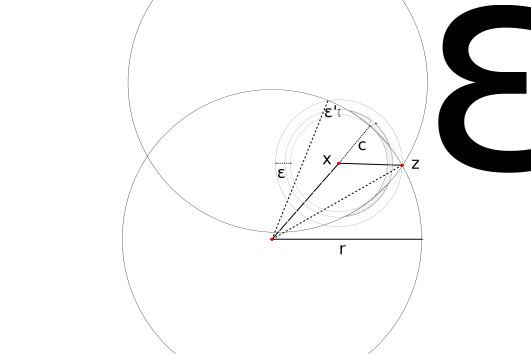
\includegraphics[height=0.55\textwidth, width=0.55\textheight]{Zeichnung2.pdf}
\end{center}
\end{figure}
The uniform interior sphere condition respectively the twin tangent ball condition implies that $\partial\Omega$  is separated by the surface of a ball of radius $r(\partial\Omega)$ from the ball $B_{c}(x)$, as seen in the graphic above of a two dimensional cut of this situation. Using this property, the graphic and a little exercise in trigonometry, one can estimate that the maximal distance another element $z_{\hat{\epsilon}}$ with $\hat{\epsilon}<\epsilon$, would have to have to $z_\epsilon$ is smaller than $\epsilon$. Therefore $(z_\epsilon)_{(r-\delta)>\epsilon>0}$ is a Cauchy-net and converges to an element $z\in\partial\Omega$. The uniqueness follows from the same estimate.
\end{proof}
\begin{remark} If $\Omega$ is a $C^k$-Jordan domain with $k\geq 1$ then we also get the inverse of the above proposition, because the unique closest point to $x\pm\frac{r(\partial\Omega)}{2}$ would have to be $x$ for $x\in\partial\Omega$, since $x-\omega(x)$ is perpendicular to the tangent space at $x$ and $\hat{\phi}$ is invertible.\end{remark}
\begin{remark} We are now able to decide up to a positive real number $\epsilon$ whether we are inside $\Omega$ or in $\Omega^c$ or in $B_\epsilon(\partial\Omega)$. In other words we know that a $C^k$-Jordan domain is coherent. This enables us to prove that the surface projection $\omega$ even exists on the whole $B_{r(\partial\Omega)}(\partial\Omega)$.\end{remark}








\chapter{Additional Results}
\begin{theorem} Let $\partial\Omega$ be a Jordan manifold that admits the twin tangent ball condition, then $\partial\Omega$ is a $C^k$-Jordan manifold if $\partial\Omega$ is $C^{k+1}$-diffeomorphic to the sphere $S$ (i.e. there exists a $r>0$ and a $C^{k+1}$-diffeomorphism $\psi:B_r(S)\rightarrow B_r(\partial\Omega)$ such that $\psi|_S=\phi$).\end{theorem}
\begin{proof}
We have to show that there exists $r(\partial\Omega)>0$ such that $\hat{\phi}(x)=\psi(\frac{x}{|x|})+(1-|x|)n(\psi(\frac{x}{|x|}))$ for $x\in B_{r(\partial\Omega)}(S)$ is a $C^k$-diffeomorphism. First of all the above expression is a composition of $C^k$-functions, and therefore itself a $C^k$ function. \\
\\
Define $\hat{\phi}^{-1}(x)=\psi^{-1}\circ\omega(x)-\langle n\circ\omega(x),x-\omega(x)\rangle \psi^{-1}\circ\omega(x)$ and observe that this is indeed the inverse of $\hat{\phi}$ defined above: If we choose $r(\partial\Omega)<r(\partial\Omega)$, where $r(\partial\Omega)$ is the constant from the twin tangent ball condition, we get the existence of the surface projection $\omega$ and furthermore that $\omega(\psi(\frac{x}{|x|})+(1-|x|)n(\psi(\frac{x}{|x|}))=\psi(\frac{x}{|x|}))$ for $x\in B_{r(\partial\Omega)}(S)$, which immediately implies that $\hat{\phi}^{-1}\circ\hat{\phi}=Id$.\\
\\
On the other hand we know that $S$ fulfills a twin tangent ball condition for any $r(S)<1$, therefore by the same argument we get that $\hat{\phi}\circ\hat{\phi}^{-1}=Id$
\\
\\
It remains to show that $\hat{\phi}^{-1}$ is a $C^k$-function and the only thing that is missing is the differentiability of $\omega$: Choose a chart $\zeta$ of $S$ with domain $V$ and image $L=(0,1)^{n-1}$\footnote{A chart is the restriction of a $C^k$ diffeomorphism between $B_s(V)$ and \\$B_s(L)\subset \mathbb{R}^{n-1}\times\mathbb{R}$, where $s>0$.} and consider the function $T:L\times(-r,r)\rightarrow B_r(\partial\Omega)$ defined by $T(x,\lambda)=\psi\circ\zeta^{-1}(x)+\lambda n(\psi\circ\zeta^{-1}(x))$ for $\lambda\in (-r,r)$ and $x\in L$.\\
\\
Obviously $\omega(x)=\psi\circ\zeta^{-1}( (T^{-1}(x))_1)$ for $x\in \omega^{-1}(V)$, where $()_1$ denotes the projection onto the first $n-1$ components, and therefore in order to study the differentiability of $\omega$ it suffices to study the differentiability of $T^{-1}$: \\
\\
Denote the derivative with respect to the variables of $L$ by $D_{\phi}$ and the derivative with respect to the variable of $(-r,r)$ by $D_\lambda$.
\begin{equation*} DT(x,\lambda)=(D_\phi T,D_\lambda T)=(D_\phi(\psi\circ\zeta^{-1}(x))+\lambda D_\phi(n(\psi\circ\zeta^{-1}(x))),n(\psi\circ\zeta^{-1}(x)))\end{equation*}
Next we need to show that $Q(x)=(D_\phi(\psi\circ\zeta^{-1}(x)),n(\psi\circ\zeta^{-1}(x)))^{-1}$ exists and is continuous:\\
\\
We know that $D(\psi(r\zeta^{-1}(x)))=(D_\phi(\psi(r\zeta^{-1}(x))),D_r(\psi(r\zeta^{-1}(x))))$ is invertible for every $(x,r)\in L\times (1-r,1+r)$. Let's denote the inverse, which is continuous on $L\times (1-r,1+r)$ by $\hat{Q}(x,1)$. Now replace the last row of $\hat{Q}$ by $\frac{n\circ\psi\circ\zeta^{-1}(x)}{|n\circ\psi\circ\zeta^{-1}(x)|^2}$ and observe that now $\hat{Q}\circ(D_\phi(\psi\circ\zeta^{-1}(x)),n(\psi\circ\zeta^{-1}(x)))$ equals the unit matrix everywhere except in the last row, since $n(\psi\circ\zeta^{-1}(x))\bot D_\phi(\psi\circ\zeta^{-1}(x))$, where the lowest entry is 1. Multiplication by $(n-1)$ elementary matrices with continuous entries therefore yields our desired continuous $Q$.\\
\\
Now observe the following equation:
\begin{equation*}Q(x)\circ DT(x,\lambda)=id-\lambda Q(x)\circ (D_\phi(n(\psi\circ\zeta^{-1}(x))),0)\end{equation*}
If we choose $r(\partial\Omega)$ smaller than $\frac{(\sup_{x\in\partial\Omega} |(Q(\zeta\circ\psi^{-1}(x))\circ (D\phi(n(x)),ß))|_\infty)^{-1}}{2}$ we are guaranteed using the geometric series technique that the inverse of $Q(x)\circ DT(x,\lambda)$ exists and therefore the inverse of $DT(x,\lambda)$ exists and is continuous since we have the general estimate:
\begin{equation*}|(id-A)^{-1}-(id-B)^{-1}|_\infty\leq |(id-A)^{-1}|_\infty|(id-B)^{-1}|_\infty|A-B|_\infty\end{equation*}
and from the geometric series technique we know that the norm of $|(id-A)^{-1}|_\infty\leq\frac{1}{1-|A|}$ if $|A|<1$.\\
\\
Finally we show that for each $x\in L\times (-r,r)$ the resulting $(DT)^{-1}(x)$ is indeed the derivative of $T^{-1}$ at $T(x)$: Let $\epsilon>0$,  
$z_1,z_2\in L\times (-r,r)$, such that $|z_1-z_2|<\delta(\epsilon)$, where $\delta$ is the modulus of differentiability of $T$, and $x=T(z_1)$, $y=T(z_2)$ then we get:
\begin{align*}&|T^{-1}(x)-T^{-1}(y)-(DT(T^{-1}(x)))^{-1}(x-y)|\\&=|DT(z_1)^{-1}\circ DT(z_1)(z_1-z_2-(DT(z_1)^{-1}(T(z_1)-T(z_2))))|\\
&\leq|DT(z_1)^{-1}|_\infty| DT(z_1)(z_1-z_2)-(T(z_1)-T(z_2)))|\leq |DT(z_1)^{-1}|_\infty \epsilon |z_1-z_2|\\
&=|DT(z_1)^{-1}|_\infty \epsilon |T^{-1}(x)-T^{-1}(y)|\end{align*}
We know see that if we are able to show that $T^{-1}$ is at least locally Lipschitz continuous, we get our desired result: We can use the fundamental theorem of calculus as in Proposition 3.2 to get for each $x,y\in\omega^{-1}(V)$ the estimate:
\begin{equation*} |\zeta\circ\psi^{-1}(x)-\zeta\circ\psi^{-1}(y)|\leq C |x-y|\end{equation*}
where $C>0$ is only dependent on $V$. If we choose $x,y\in\omega^{-1}(V)$, such that $|x-y|< \delta_n(\epsilon)$, where $\delta_n$ is the modulus of continuity of the inner normal function $n:\partial\Omega\rightarrow\mathbb{R}^n$, then we get for $\lambda,\hat{\lambda}\in (-r,r)$:
\begin{equation*} |x-y|\leq \hat{C}|(x+\lambda n(x))-(y+\hat{\lambda} n(y))|\end{equation*}
\end{proof}

\begin{proof} 
Let $x\in\mathbb{R}^n$. Then using the proof of last lemma we can construct a Cauchy sequence $(y_k)_{k\geq 1}\subset\mathbb{R}^n$, such that if $|x-\partial\Omega|<\frac{1}{2k}$ then $y_k=x$ otherwise if $|x-\partial\Omega|>\frac{1}{2k+1}$ we can, since we can decide whether $x\in\Omega$ or $x\in\Omega^c$,  use the proof of Proposition 3.4 on $\Omega$ respectively $\Omega^c$. We get that $|u_n-u_m|<\frac{1}{n}$ for $m\geq n$ and therefore this is indeed a Cauchy sequence and we can set $\omega(x)=\lim_ky_k$.
\\
\\
Let $x\in B_r(\partial\Omega)$ then for any $v$ in the tangent space $T_x(\partial\Omega)$ we get $\langle v, x-\omega(x)\rangle= 0$, since if there would exists a $v$ such that $x\in B_r(\partial\Omega)$, we could found a $y\in\partial\Omega$ such that $|x-y|<|x-\partial\Omega$.\\
\\
Therefore we can write $x=\omega(x)+\langle n(\omega(x)),x-\omega(x)\rangle n(\omega(x))$, which shows, since $-r(\partial\Omega)<\langle n(x),x-\omega(x)\rangle<r(\partial\Omega)$,  that 
$\omega(x)=\phi(\frac{\hat{\phi}^{-1}(x)}{|\hat{\phi}^{-1}(x)|})$. The result follows since this representation is a $C^k$-function.
%By assumption the map $\hat{\phi}$ is a $C^{k}$-function, just like its inverse. Denote by $T$ the Diffeomorphism defined by $T(x)=(\frac{x}{|x|},1-|x|)$ for $x\in B_{r(\partial\Omega)}(S)$, identifying the annullus $B_{r(\partial\Omega)}(S)$ with the cylinder $S\times(-r,r)$.  We just have to show that the inverse of $\hat{\phi}\circ T$ coincides with $(\phi^{-1}\circ\omega_{\partial\Omega},|.-\parital\Omega|)$, which shows that $\omega_{\partial\Omega}$ is just the projection onto the first $n-1$ coordinates of $\hat{\phi}\circ T^{-1}\circ\hat{\phi}^{-1}$, therefore a $C^{k}$-function:\\
%\\
%The only thing we have to show is that through the function $\hat{\phi}$ the surface projection $\omega_{S}(x)$ with respect to $S$ of an element $x\in B_r(S)$ will be mapped onto the surface projection $\omega_{\partial\Omega}(x)$ with respect to $\partial\Omega$ and that the corresponding property holds also for $\hat{\phi}^{-1}$. This follows immediately from the fact that straight lines perpendicular to $S$ correspond through $\hat{\phi}$ to straight lines perpendicular to $\partial\Omega$ and since the line between an element and its surface projection is perpendicular to the surface.
\end{proof}